% Preview source code

%% LyX 2.1.3 created this file.  For more info, see http://www.lyx.org/.
%% Do not edit unless you really know what you are doing.
\documentclass[12pt,british,a4paper,ruled,noend,slide]{article}
\renewcommand{\sfdefault}{lmss}
\renewcommand{\ttdefault}{lmtt}
\usepackage[utf8]{inputenc}
\usepackage[T1]{fontenc}
\usepackage{lmodern}
\usepackage[scaled]{beramono}
%\synctex=-1
\usepackage{babel}
\usepackage{varioref}
\usepackage{prettyref}
\usepackage{booktabs}
\usepackage{pdflscape}
\usepackage{mathtools}
\usepackage{algorithm2e}
\usepackage{amsmath}
\usepackage{amssymb}
\usepackage{graphicx}
\usepackage[unicode=true,
 bookmarks=true,bookmarksnumbered=false,bookmarksopen=false,
 breaklinks=true,pdfborder={0 0 0},backref=page,colorlinks=false]
 {hyperref}
\hypersetup{pdftitle={CMOS Calculator},
 pdfauthor={Joshua Clark}}

\makeatletter

%%%%%%%%%%%%%%%%%%%%%%%%%%%%%% LyX specific LaTeX commands.
%% Because html converters don't know tabularnewline
\providecommand{\tabularnewline}{\\}
\renewcommand{\arraystretch}{1.2}

%%%%%%%%%%%%%%%%%%%%%%%%%%%%%% Textclass specific LaTeX commands.
\newcommand{\code}[1]{\texttt{#1}}

%%%%%%%%%%%%%%%%%%%%%%%%%%%%%% User specified LaTeX commands.
% Preview source code

\usepackage{babel}
% Preview source code

\usepackage{multicol}
\usepackage{tikz}
\usetikzlibrary{calc}
\usepackage{listings}

\lstdefinelanguage{scala}{
  morekeywords={%
          abstract,case,catch,class,def,do,else,extends,%
          false,final,finally,for,forSome,if,implicit,import,lazy,%
          match,new,null,object,override,package,private,protected,%
          return,sealed,super,this,throw,trait,true,try,type,%
          val,var,while,with,yield},
  otherkeywords={=>,<-,<\%,<:,>:,\#,@},
  sensitive=true,
  morecomment=[l]{//},
  morecomment=[n]{/*}{*/},
  morestring=[b]",
  morestring=[b]',
  morestring=[b]"""
}[keywords,comments,strings]
 
% activate the language and predefine settings
\lstset{language=Scala}

% Other listings-related settings from
% http://lampsvn.epfl.ch/trac/scala/export/26099/scala-tool-support/trunk/src/latex/scaladoc.sty
% activate the language and predefine settings
\lstset{
    language=Scala,%
    xleftmargin=4mm,%
    frame=top,frame=bottom,
    aboveskip=3mm,%
    belowskip=3mm,%
    fontadjust=true,%
    columns=[c]fixed,%
    keepspaces=true,%
    basewidth={0.58em, 0.53em},%
    tabsize=2,%
    basicstyle=\renewcommand{\baselinestretch}{0.95}\scriptsize\ttfamily,%
    commentstyle=\itshape,%
    keywordstyle=\bfseries,%
    mathescape=true,%
    escapechar=`,%
    captionpos=t,%
    framerule=0.3pt,%
    firstnumber=0,%
    numbersep=5pt,%
    numberstyle=\tiny,%
    flexiblecolumns,
    breaklines,
	stepnumber=5,
	numbers=left,
	showstringspaces=false
}
 
\lstdefinestyle{floating}{%
    xleftmargin=10pt,%
    xrightmargin=5pt,%
    aboveskip=4mm,%
    belowskip=4mm,%
    fontadjust=true,%
    columns=[c]flexible,%
    keepspaces=true,%
    basewidth={0.5em, 0.425em},%
    tabsize=2,%
    basicstyle=\renewcommand{\baselinestretch}{0.95}\ttfamily,%
    commentstyle=\rm,%
    keywordstyle=\bfseries,%
    mathescape=true,%
    captionpos=b,%
    framerule=0.3pt,%
    firstnumber=0,%
    numbersep=1.5mm,%
    numberstyle=\tiny,%
    float=tbp,%
    frame=tblr,%
    framesep=5pt,%
    framexleftmargin=3pt,%
    abovecaptionskip=\smallskipamount,%
    belowcaptionskip=\smallskipamount,%
} % to define: caption, label


\setlength{\unitlength}{0.4cm}

% standard gates are picture (6,6)
% with connections at (-6,-1), (-6,1) and (0,0)
% inverters are (5,2) connected at (-5,0) and (0,0)
% big inverters are (10,4) connected at (-10,0) and (0,0)
% downward inverters are (2,5) connected at (0,5) and (0,0)

\newcommand{\notgate}{\begin{picture}(5,2)(5,0)
        \put(0,0){\line(1,0){2}}
                \put(2,-1){\line(0,1){2}}
                \put(2,-1){\line(2,1){2}}
                \put(2,1){\line(2,-1){2}}
                \put(4.25,0){\circle{0.5}}
        \put(4.5,0){\line(1,0){0.5}}
\end{picture}}

\newcommand{\buffgate}{\begin{picture}(5,2)(5,0)
        \put(0,0){\line(1,0){2}}
        \begin{thicklines}
                \put(2,-1){\line(0,1){2}}
                \put(2,-1){\line(2,1){2}}
                \put(2,1){\line(2,-1){2}}
        \end{thicklines}
        \put(4,0){\line(1,0){1}}
\end{picture}}

\newcommand{\revnotgate}{\begin{picture}(5,2)(0,0)
        \put(5,0){\line(-1,0){2}}
        \begin{thicklines}
                \put(3,-1){\line(-0,1){2}}
                \put(3,-1){\line(-2,1){2}}
                \put(3,1){\line(-2,-1){2}}
                \put(0.75,0){\circle{0.5}}
        \end{thicklines}
        \put(0.5,0){\line(-1,0){0.5}}
\end{picture}}

\newcommand{\bignotgate}{\begin{picture}(10,2)(10,0)
        \put(0,0){\line(1,0){4}}
        \begin{thicklines}
                \put(4,-2){\line(0,1){4}}
                \put(4,-2){\line(2,1){4}}
                \put(4,2){\line(2,-1){4}}
                \put(8.25,0){\circle{0.5}}
        \end{thicklines}
        \put(8.5,0){\line(1,0){1.5}}
\end{picture}}

\newcommand{\downnotgate}{\begin{picture}(2,5)(0,-5)
        \put(0,0){\line(0,-1){2}}
        \begin{thicklines}
                \put(-1,-2){\line(1,0){2}}
                \put(-1,-2){\line(1,-2){1}}
                \put(1,-2){\line(-1,-2){1}}
                \put(0,-4.25){\circle{0.5}}
        \end{thicklines}
        \put(0,-4.5){\line(0,-1){0.5}}
\end{picture}}

% \newcommand\inverter{\begin{picture}(6,6)
%       \put(0,-2.25){\line(0,1){4.5}}
%       \put(0,-2.25){\line(4,3){2.7}}
%       \put(0,2.25){\line(4,-3){2.7}}
%       \begin{thicklines}
%               \put(3,0){\circle{0.75}}
%       \end{thicklines}
%       \put(6,0){\line(-1,0){2.625}}
% \end{picture}}

\newcommand{\andgate}{\begin{picture}(6,6)(6,0)  
        \multiput(0,-1)(0,2){2}{\line(1,0){1}}
        \begin{thicklines}
                \put(1,-2){\line(0,1){4}}
                \put(1,0){\oval(8,4)[r]}
        \end{thicklines}
        \put(5,0){\line(1,0){1}}
\end{picture}}

\newcommand{\rightandgate}{\begin{picture}(6,6)(6,0)  
        \put(0,0){\line(1,0){1}}
        \begin{thicklines}
                \put(1,-2){\line(0,1){4}}
                \put(1,0){\oval(8,4)[r]}
        \end{thicklines}
        \put(5,0){\line(1,0){1}}
\end{picture}}

\newcommand{\nandgate}{\begin{picture}(6,6)(6,0)  
        \multiput(0,-1)(0,2){2}{\line(1,0){1}}
        \begin{thicklines}
                \put(1,-2){\line(0,1){4}}
                \put(1,0){\oval(8,4)[r]}
                \put(5.25,0){\circle{0.5}}
        \end{thicklines}
        \put(5.5,0){\line(1,0){0.5}}
\end{picture}}

\newcommand{\orgate}{\begin{picture}(6,6)(6,0)  
        \multiput(0,-1)(0,2){2}{\line(1,0){1.7}}
        \begin{thicklines}
                \qbezier(1,2)(3,0)(1,-2)
                \qbezier(1,2)(4,2)(5,0)
                \qbezier(1,-2)(4,-2)(5,0)
        \end{thicklines}
        \put(5,0){\line(1,0){1}}
\end{picture}}

\newcommand{\leftorgate}{\begin{picture}(6,6)(-6,0)  
        \multiput(0,-1)(0,2){2}{\line(-1,0){1.7}}
        \begin{thicklines}
                \qbezier(-1,2)(-3,0)(-1,-2)
                \qbezier(-1,2)(-4,2)(-5,0)
                \qbezier(-1,-2)(-4,-2)(-5,0)
        \end{thicklines}
        \put(-5,0){\line(-1,0){1}}
\end{picture}}

\newcommand{\downorgate}{\begin{picture}(6,6)(3,0)
        % \multiput(-1,6)(2,0){2}{\line(0,-1){1.7}}
        \begin{thicklines}
                \qbezier(-2,5)(-2,2)(0,1)
                \qbezier(2,5)(2,2)(0,1)
                \qbezier(-2,5)(0,3)(2,5)
        \end{thicklines}
        \put(0,0){\line(0,1){1}}
\end{picture}}

\newcommand{\norgate}{\begin{picture}(6,6)(6,0)  
        \multiput(0,-1)(0,2){2}{\line(1,0){1.7}}
        \begin{thicklines}
                \qbezier(1,2)(3,0)(1,-2)
                \qbezier(1,2)(4,2)(5,0)
                \qbezier(1,-2)(4,-2)(5,0)
                \put(5.25,0){\circle{0.5}}
        \end{thicklines}
        \put(5.5,0){\line(1,0){0.5}}
\end{picture}}

\newcommand{\leftnorgate}{\begin{picture}(6,6)(-6,0)  
        \multiput(0,-1)(0,2){2}{\line(-1,0){1.7}}
        \begin{thicklines}
                \qbezier(-1,2)(-3,0)(-1,-2)
                \qbezier(-1,2)(-4,2)(-5,0)
                \qbezier(-1,-2)(-4,-2)(-5,0)
                \put(-5.25,0){\circle{0.5}}
        \end{thicklines}
        \put(-5.5,0){\line(-1,0){0.5}}
\end{picture}}

\newcommand{\xnorgate}{\begin{picture}(6,6)(6,0)  
        \multiput(0,-1)(0,2){2}{\line(1,0){1.5}}
        \begin{thicklines}
                \qbezier(0.8,1.9)(2.8,0)(0.8,-1.9)
                \qbezier(1.3,2)(3.0,0)(1.3,-2)
                \qbezier(1.3,2)(4,2)(5,0)
                \qbezier(1.3,-2)(4,-2)(5,0)
                \put(5.25,0){\circle{0.5}}
        \end{thicklines}
        \put(5.5,0){\line(1,0){0.5}}
\end{picture}}

\newcommand{\xorgate}{\begin{picture}(6,6)(6,0)  
        \multiput(0,-1)(0,2){2}{\line(1,0){1.5}}
        \begin{thicklines}
                \qbezier(0.8,1.9)(2.8,0)(0.8,-1.9)
                \qbezier(1.3,2)(3.0,0)(1.3,-2)
                \qbezier(1.3,2)(4,2)(5,0)
                \qbezier(1.3,-2)(4,-2)(5,0)
        \end{thicklines}
        \put(5,0){\line(1,0){1}}
\end{picture}}

\newcommand{\majgate}{\begin{picture}(6,6)(6,0)  
        \multiput(0,-1)(0,1){3}{\line(1,0){1}}
        \begin{thicklines}
                \put(1,-2){\line(0,1){4}}
                \multiput(1,-2)(0,4){2}{\line(1,0){3}}
                \put(4,0){\oval(2,4)[r]}
        \end{thicklines}
        \put(3,0){\makebox(0,0){\strut\textit{maj}}}
        \put(5,0){\line(1,0){1}}
\end{picture}}


\newcommand{\Celem}{\begin{picture}(6,6)(6,0)  
        \put(0,-1){\line(3,1){1.60}}
        \put(0,1){\line(3,-1){1.60}}
        \begin{thicklines} \put(3,0){\circle{3}} \put(3,0){\makebox(0,0){\textsc{c}}} \end{thicklines}
        \put(6,0){\line(-1,0){1.5}}
\end{picture}}

\newcommand{\Celemup}{\begin{picture}(6,6)(0,6)  
        \put(-1,0){\line(1,3){0.53}}
        \put(1,0){\line(-1,3){0.53}}
        \begin{thicklines}
                \put(0,3){\circle{3}}
                \put(0,3){\makebox(0,0){\textsc{c}}}
        \end{thicklines}
        \put(0,6){\line(0,-1){1.5}}
\end{picture}}

\newcommand{\Celemdown}{\begin{picture}(6,6)(0,0)  
        \put(-1,6){\line(1,-3){0.53}}
        \put(1,6){\line(-1,-3){0.53}}
        \begin{thicklines}
                \put(0,3){\circle{3}}
                \put(0,3){\makebox(0,0){\textsc{c}}}
        \end{thicklines}
        \put(0,0){\line(0,1){1.5}}
\end{picture}}

% standard flipflops are picture (10,10)
% with connections at (0,7), (1,3) and at (10,3) and (10,7)

\newcommand{\dtype}{\begin{picture}(10,10)(0,0)  
        \put(1,3){\line(1,0){1}}
        \put(0,7){\line(1,0){2}}
        \multiput(8,3)(0,4){2}{\line(1,0){2}}
        \begin{thicklines}
                \put(2,1){\framebox(6,8){}}
        \end{thicklines}
        \put(2,3){\makebox(0,0)[l]{$\mskip-2mu>$}}
        \put(2,7){\makebox(0,0)[l]{\textsc{\strut\,d}}}
        \put(8,7){\makebox(0,0)[r]{\textsc{\strut q\,}}}
        \put(8,3){\makebox(0,0)[r]{\textsc{\strut \=q\,}}}
\end{picture}}

\newcommand{\ttype}{\begin{picture}(10,10)(0,0)  
        \put(1,3){\line(1,0){1}}
        \put(0,7){\line(1,0){2}}
        \multiput(8,3)(0,4){2}{\line(1,0){2}}
        \begin{thicklines}
                \put(2,1){\framebox(6,8){}}
        \end{thicklines}
        \put(2,3){\makebox(0,0)[l]{$\mskip-2mu>$}}
        \put(2,7){\makebox(0,0)[l]{\textsc{\strut\,t}}}
        \put(8,7){\makebox(0,0)[r]{\textsc{\strut q\,}}}
        \put(8,3){\makebox(0,0)[r]{\textsc{\strut \=q\,}}}
\end{picture}}

\newcommand{\leveldtype}{\begin{picture}(10,10)(0,0)  
        \put(1,3){\line(1,0){1}}
        \put(0,7){\line(1,0){2}}
        \multiput(8,3)(0,4){2}{\line(1,0){2}}
        \begin{thicklines}
                \put(2,1){\framebox(6,8){}}
        \end{thicklines}
        \put(2,2.8){\framebox(0.6,0.4)[l]{}}
        \put(2,7){\makebox(0,0)[l]{\textsc{\strut\,d}}}
        \put(8,7){\makebox(0,0)[r]{\textsc{\strut q\,}}}
        \put(8,3){\makebox(0,0)[r]{\textsc{\strut \=q\,}}}
\end{picture}}





% standard transistors are picture (4.5,6)
% with connections at (0,-3), (0,3) and gate at (-4.5,0)

\newcommand{\sntrans}{{\begin{picture}(4.5,8)(-4.5, -3)
        \put(-4.5,0){\line(1,0){2.25}}
        \put(-2.25,-1.5){\line(0,1){3}}
        \begin{thicklines}
                \put(-1.5,-1.5){\line(0,1){3}}
        \end{thicklines}
        \put(0,-3){\line(0,1){1.5}}
        \put(0,-1.5){\line(-1,0){1.5}}
        \put(0,1.5){\line(-1,0){1.5}}
        \put(0,3){\line(0,-1){1.5}}
        \put(1,-3){$d$}
        \put(1,3){$s$}
\put(-5.5,0){$g$}
\end{picture}}}

\newcommand{\ntrans}{{\begin{picture}(4.5,6)(0,0)
        \put(-4.5,0){\line(1,0){2.25}}
        \put(-2.25,-1.5){\line(0,1){3}}
        \begin{thicklines}
                \put(-1.5,-1.5){\line(0,1){3}}
        \end{thicklines}
        \put(0,-3){\line(0,1){1.5}}
        \put(0,-1.5){\line(-1,0){1.5}}
        \put(0,1.5){\line(-1,0){1.5}}
        \put(0,3){\line(0,-1){1.5}}
\end{picture}}}

\newcommand{\ntransdown}{{\begin{picture}(6,4.5)(0,0) 
        \put(0,-4.5){\line(0,1){2.25}}
        \put(1.5,-2.25){\line(-1,0){3}}
        \begin{thicklines}
                \put(1.5,-1.5){\line(-1,0){3}}
        \end{thicklines}
        \put(3,0){\line(-1,0){1.5}}
        \put(-1.5,0){\line(0,-1){1.5}}
        \put(1.5,0){\line(0,-1){1.5}}
        \put(-3,0){\line(1,0){1.5}}
\put(0,-4){$d$}
        \put(0,4){$s$}
\put(-5.5,0){$g$}
\end{picture}}}

\newcommand{\ntransup}{{\begin{picture}(6,4.5)(0,0)
        \put(0,4.5){\line(0,-1){2.25}}
        \put(-1.5,2.25){\line(1,0){3}}
        \begin{thicklines}
                \put(-1.5,1.5){\line(1,0){3}}
        \end{thicklines}
        \put(-3,0){\line(1,0){1.5}}
        \put(-1.5,0){\line(0,1){1.5}}
        \put(1.5,0){\line(0,1){1.5}}
        \put(3,0){\line(-1,0){1.5}}
\end{picture}}}

\newcommand{\sptrans}{{\begin{picture}(4.5,6)(-4.5,-3) 
        \put(-4.5,0){\line(1,0){1.5}}
        \put(-2.625,0){\circle{0.75}}
        \put(-2.25,-1.5){\line(0,1){3}}
        \begin{thicklines}
                \put(-1.5,-1.5){\line(0,1){3}}
        \end{thicklines}
        \put(0,-3){\line(0,1){1.5}}
        \put(0,-1.5){\line(-1,0){1.5}}
        \put(0,1.5){\line(-1,0){1.5}}
        \put(0,3){\line(0,-1){1.5}}
\put(1,-3){$d$}
        \put(1,3){$s$}
\put(-5.5,0){$g$}
\end{picture}}}

\newcommand{\ptrans}{{\begin{picture}(4.5,6)(0,0) 
        \put(-4.5,0){\line(1,0){1.5}}
        \put(-2.625,0){\circle{0.75}}
        \put(-2.25,-1.5){\line(0,1){3}}
        \begin{thicklines}
                \put(-1.5,-1.5){\line(0,1){3}}
        \end{thicklines}
        \put(0,-3){\line(0,1){1.5}}
        \put(0,-1.5){\line(-1,0){1.5}}
        \put(0,1.5){\line(-1,0){1.5}}
        \put(0,3){\line(0,-1){1.5}}
\end{picture}}}

\newcommand{\ptransup}{{\begin{picture}(6,4.5)(0,0)
        \put(0,4.5){\line(0,-1){1.5}}
        \put(0,2.625){\circle{0.75}}
        \put(-1.5,2.25){\line(1,0){3}}
        \begin{thicklines}
                \put(-1.5,1.5){\line(1,0){3}}
        \end{thicklines}
        \put(-3,0){\line(1,0){1.5}}
        \put(-1.5,0){\line(0,1){1.5}}
        \put(1.5,0){\line(0,1){1.5}}
        \put(3,0){\line(-1,0){1.5}}
\end{picture}}}

\newcommand{\ptransdown}{{\begin{picture}(6,4.5)(0,0) 
        \put(0,-4.5){\line(0,1){1.5}}
        \put(0,-2.625){\circle{0.75}}
        \put(1.5,-2.25){\line(-1,0){3}}
        \begin{thicklines}
                \put(1.5,-1.5){\line(-1,0){3}}
        \end{thicklines}
        \put(3,0){\line(-1,0){1.5}}
        \put(-1.5,0){\line(0,-1){1.5}}
        \put(1.5,0){\line(0,-1){1.5}}
        \put(-3,0){\line(1,0){1.5}}
\end{picture}}}

\usepackage{multirow}
\begin{filecontents*}{logexp.tex}
\begin{tabular}{cc|cccc}
 & \multicolumn{1}{c}{} & \multicolumn{4}{c}{$ab$}\tabularnewline
 &  & 00 & 01 & 11 & 10\tabularnewline
\hline 
\multirow{2}{*}{$c$} & 0 & 0 & 0 & 1 & 0\tabularnewline
 & 1 & 1 & 0 & 1 & 0\tabularnewline
\end{tabular}
\end{filecontents*}

\begin{filecontents*}{xortab.tex}
\begin{tabular}{cc|cccc}
 & \multicolumn{1}{c}{} & \multicolumn{4}{c}{$ab$}\tabularnewline
 &  & 00 & 01 & 11 & 10\tabularnewline
\hline 
\multirow{2}{*}{$c$} & 0 & 0 & 1 & 0 & 1\tabularnewline
 & 1 & 1 & 0 & 1 & 0\tabularnewline
\end{tabular}
\end{filecontents*}

\newcommand{\blob}{{\circle*{0.4}}}
\usepackage{xfrac}
\usepackage[protrusion=true,expansion=true,kerning=true,tracking=true,spacing=true]{microtype}
\usepackage{tabularx}
\usepackage{cleveref}






\makeatother

\begin{document}
\thispagestyle{empty} 

\begin{center}
\begin{minipage}[c]{0.75\linewidth}%
 \centering %University logo

\includegraphics[width=0.4\linewidth]{oxford} 

\vspace{2cm}
 %Thesis title 
{\uppercase{\Large{}CMOS Calculator }{\Large \par}} \vspace{2cm}
%Author's name 
{\Large{}Joshua Clark}{\Large \par}

\vspace{2cm}
%Degree 
{\Large{}Third Year Project Report for the Final Honour School of Computer Science}{\Large \par}

 \vspace{2cm}
 %Date 
{\Large{}May 2015} %
\end{minipage}
\par\end{center}

\clearpage{}
\begin{abstract}
The aim of this project was to build a CMOS simulator, with the following
interactive elements: 
\begin{itemize}
\item Simplification and CMOS implementation of arbitrary logical expressions 
\item Simulation to visualise the change in flow of potential as the state
of inputs changed 
\item Simulation of delay in propagation of state for large networks. 
\end{itemize}
There are many tools in existence to design CMOS circuits, but most
focus on the physical implementation and the exact positioning of
transistors, rather than a more abstract approach, as may be required
when reasoning about the layout of circuits, this tool seeks to remedy
that issue. It quickly became apparent that the approach that I was
using had various similarities to a compiler, which will be a focus
of this document. Additionally, this report will discuss alternative
approaches not used in the final implementation to produce the final
CMOS output. 
\end{abstract}
\tableofcontents{}

\listofalgorithms

\listoffigures

\section{Introduction}

The idea of logical functions is familiar to many, and even a schoolchild
can grasp the concept of a box receiving true/false inputs and producing
a true/false output, and lots of these boxes in interesting combinations
can yield more interesting functions. Through introducing these concepts,
and producing more and more intricate diagrams, they can then see
how more complicated ideas, such as addition and subtraction are implemented,
and maybe how these are used in the modern computers used today. However,
what is rarely discussed is what is inside these boxes: they are usually
presented as the lowest level inputs and treated as the basic building
blocks. The layer underneath this is built up of Complementary Metal-Oxide
Semiconductors, henceforth referred to as CMOS. The treatment of this
document mainly concerns producing this sequence of transistors from
plain string through a series of intermediary formats, until a visual
representation is produced.

Initially, this document will define key concepts, such as the fundamental
propositional logic syntax and semantic meanings usually associated
with logic gates, and the definition of the two different transistors
that form CMOS. We will then go on to discuss the requirements and
use cases of a program to present these ideas before defining the
algorithms to be used. On closer inspection, their composition has
a behaviour not entirely dissimilar to that of a compiler, and the
subsequent design of the program upon realising this was the paradigm
being used will then be analysed. The program that has then been produced
will finally be compared against the stated objectives, with possible
further work then listed.

Projects of a much greater scope already exist in the real world, for example,
the third iteration of the Simulation Program with Integrated Circuit Emphasis
(SPICE3) simulates circuits with up to 43 different types of transistor,
however, requires a specifically formatted input that is rather difficult to
read for new users.  There are also many Very-large-scale integration programs,
which deal with CMOS, however, as the name suggests, thsee are more appropriate
for large projects, such as CPU design.  As previously discussed, there are also
many applications where you may use logic gates to implement larger functions,
however, these rarely include details about the transistors used.

This program will attempt to combine the ease of use of simple logical expressions
while producing an easily understandable representation of the output needed.  As such,
it will not concern itself with the precise layout of wires between the different inputs.

\subsection{Typical Use}

On starting the application, the user will typically enter a well-formed
logical expression, as described using the grammar above, with a non-trivial
canonical representation (i.e.\ $\mathit{expr}\neq\top,\bot$). This
will then be parsed and converted to a canonical form (DNF) which
will then be processed to produce a series of transistors to implement
the desired logical expression. This will then be rendered, with gates
highlighted red to indicate drivenness, and a list of variables provided.
The user can then change the assignment of these variables by toggling
a checkbox, and this change will then be reflected in the rendered
set of gates.


\subsection{Document Conventions}

By convention, when class diagrams are used, ovals will represent
traits/abstract classes, with rectangles representing concrete implementations.
Objects are indicated using bold lines in the diagram, and are similar
in behaviour to statically declared objects in many languages.

Whenever \texttt{this font face} is used, the text is referring to
either some implementation level object or class, or the grammar used
by the parser as opposed to the standard blackboard mathematical symbols,
or text entered into the application or used for testing.

\section{Requirements and Design}



\subsection{Requirements}

The program would be expected to satisfy the following minimal requirements
in order for it to be considered successful: 
\begin{description}
\item [{Accuracy}] any representation of CMOS produced must correctly implement
the logical expression that has been entered, and the visual output
of the expression should match the model that has been stored. 
\item [{Representation}] the produced visualisation should be intuitive
to read: each element should be presented separately from the others,
and clearly labelled. Any gate carrying potential should be clearly
highlighted. 
\item [{Portability}] the visual output produced by the program should
be available to the user in a variety of formats. 
\item [{Interactivity}] the program should produce sensible warnings when
an expression that is not possible to parse has been entered. Once
a CMOS representation has been constructed, it should be possible
for the user to interact with the publicly visible inputs (the variables
named in the initial expression), with updates delivered with a minimal
amount of latency. Should the user wish to view the change in state
due to the latency of the transistors, this should be visible, and
at a variable speed. 
\end{description}
\subsection{Design}

In order to fulfil the above specifications, it was obvious that a
graphical interface would be required, so that the user could quickly
interact with the program and determine the variable assignments intuitively,
and to have their actions quickly reflected in the circuit diagram.
Initially, due to the quality of the output produced by \LaTeX{} diagrams,
using the Tikz engine to produce the output and importing temporary
files was considered, given the success of projects such as TikzEdt\cite{tikzedt},
however, as it would not be possible to assume that any system would
have the necessary libraries and programs installed, it was determined
that this would not be a feasible method to consider. Additionally,
by using a Java-based drawing library, animations would be easier,
should the project be extended to include them, as opposed to a \LaTeX{}
based solution, which is, by definition, designed for static documents.

Given the nature of the project, the model-view-controller paradigm
allows a sensible division of labour, also allowing for extensibility
and clear separation of the purpose of the model and the interface.

\begin{figure}
\begin{centering}
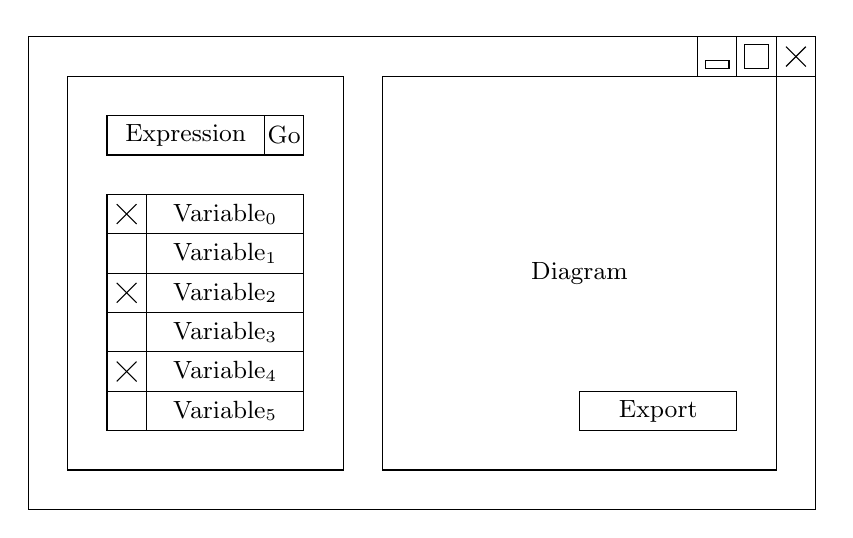
\begin{tikzpicture}[scale=1, every node/.style={scale=1,font=\small}]
\draw  (0,0) rectangle (10,6) node (v16) {};
\draw  (0.5,0.5) rectangle (4,5.5);
\draw  (4.5,0.5) rectangle (9.5,5.5) node (v15) {};
\draw  (1,5) rectangle (3,4.5);
\draw  (3,5) rectangle (3.5,4.5);
\node at (3.25,4.75) {Go};
\node at (2,4.75) {Expression};
\node at (2.5,3.75) {Variable$_0$};
\node at (2.5,3.25) {Variable$_1$};
\node at (2.5,2.75) {Variable$_2$};
\node at (2.5,2.25) {Variable$_3$};
\node at (2.5,1.75) {Variable$_4$};
\node at (2.5,1.25) {Variable$_5$};
\node at (7,3) {Diagram};
\draw  (1,4) node (v7) {} rectangle (3.5,3.5);
\draw  (1,3) node (v1) {} rectangle (3.5,3.5);
\draw  (3.5,2.5) node (v2) {} rectangle (v1);
\draw  (1,2) node (v3) {} rectangle (v2);
\draw  (3.5,1.5) node (v4) {} rectangle (v3);
\draw  (1,1) rectangle (v4);
\draw  (1.5,3.5) node (v8) {} rectangle (1,4);
\draw  (1.5,3) node (v10) {} rectangle (1,3.5) node (v5) {};
\draw  (1.5,2.5) node (v11) {} rectangle (v1);
\draw  (1.5,2) node (v13) {} rectangle (1,2.5) node (v9) {};
\draw  (1.5,1.5) node (v12) {} rectangle (1,2);
\draw  (1.5,1) rectangle (1,1.5) node (v14) {};
\node (v6) at (1.5,4) {};
\draw  (v5) edge (v6);
\draw  (v7) edge (v8);
\draw  (v9) edge (v10);
\draw  (v1) edge (v11);
\draw  (v12) edge (v3);
\draw  (v13) edge (v14);
\draw  (8.5,6) rectangle (9,5.5);
\draw  (9,6) rectangle (v15);
\draw  (9.5,6) node (v18) {} rectangle (10,5.5) node (v17) {};
\draw  (v15) edge (v16);
\draw  (v17) edge (v18);
\draw  (9.1,5.9) rectangle (9.4,5.6);
\draw  (8.6,5.7) rectangle (8.9,5.6);
\draw  (9,1) rectangle (7,1.5); \node at (8,1.25) {Export};\end{tikzpicture} 
\par\end{centering}

\caption{Initial Design}
\end{figure}





\section{Definitions}


\subsection{Logical Expressions}

A logical expression is built from a combination of constants, literals,
conjunctions, disjunctions and negations\cite{intlog}, using a grammar described
as follows:

\begin{align}
e & =\neg e=\texttt{!e}\label{eq:neg}\\
 & \mid e\lor e=\texttt{e or e}\label{eq:disj}\\
 & \mid e\land e=\texttt{e and e}\label{eq:conj}\\
 & \mid c\label{eq:cons}\\
 & \mid v\label{eq:var}\\
v & \in\Sigma\\
c & =\top\mid\bot=\texttt{0}\mid\texttt{1}
\end{align}
where $\Sigma$ is some accepted alphabet of variables (
in this program, as described by the Perl-Compatible Regex \verb&^(?!out|and|or$)([A-Za-z0-9]+)&
that is, every alphanumeric phrase, with the exception of the single
word \verb+out+, which has been reserved for specific use within
the program, and \verb+and+ and \verb+or+ which are keywords in
the logical expression language). $\top\text{ and }\bot$ are used
within this text to denote the notions true and false, respectively,
and are represented in the program by the strings \code{0} and \code{1}
respectively. Additionally, the order that the various production
rules are listed also gives an order of precedence, with negations
taking a higher precedence in the parse tree than disjunctions and conjunctions. Each variable
within the expression that is used is given an assignment by an evaluation
function, commonly called $\mathcal{A}:\mathcal{V}\rightarrow\{\top,\bot\}$\label{eq:assi},
with the set of variables typically denoted as $\mathcal{V}$. A logical
expression $E$ is then evaluated recursively based on the following
rules: 
\begin{itemize}
\item $E=F\land G$: $E$ is evaluated as true iff $F$ is true and $G$
is true (corresponding to equation \ref{eq:neg}) 
\item $E=F\lor G$: $E$ is evaluated as true iff $F$ is true or $G$ is
true (corresponding to equation \ref{eq:disj}) 
\item $E=\neg F$: $E$ is evaluated as true iff $F$ is false (corresponding
to equation \ref{eq:conj}) 
\item $E=v$ for some $v\in\Sigma$ is evaluated as true iff $\mathcal{A}(v)=\top$
(corresponding to equation \ref{eq:var}) 
\item $E=c$ for some constant is evaluated as the constant (corresponding
to equation \ref{eq:cons}) 
\end{itemize}

\subsection{CMOS Transistors}

As the name would indicate, CMOS is made up of two distinct, complementary
parts\cite{digsys}: a P-transistor can only carry high potential
from their source to their drain when the gate (connected to some
wire representing a variable) is not driven, whereas an N-transistor
can only carry low potential from their drain to their source when
the gate is driven. Two power rails then provide a low potential (commonly
referred to as $V_{dd},$ and in this document, referred to at an
implementation level as \code{Drain}), and a high potential (commonly
referred to as $V_{ss},$ and in this document, referred to at an
implementation level as \code{Source}), with a third wire used as
the output wire.

\begin{eqnarray}
P(g,s,d) & = & \neg g\rightarrow(s\leftrightarrow d)\label{eq:pgate}\\
N(g,s,d) & = & g\rightarrow(s\leftrightarrow d)\label{eq:ngate}
\end{eqnarray}


Equation \ref{eq:pgate} describes a simplified version of the P-transistor:
the potential is only carried ($s\text{ matches }d$) when the input
$g$ is not powered, losing the notion that only high potential flows
from the source to the drain. Equation \ref{eq:ngate} similarly describes
a simplified version of the N-transistor: the potential is only carried
($s\text{ matches }d$) when the input $g$ is powered, losing the
notion that only low potential flows from the drain to the source.

\begin{figure}
\begin{centering}
\sntrans \begin{picture}(4.5,6)\end{picture} \sptrans 
\par\end{centering}

\caption{N-transistor and P-transistor, respectively}
\end{figure}


Therefore, when using these transistors, it is not sufficient to specify
the implementation of a logical expression in a positive sense (carrying
potential when the valuations of the inputs causes the expression
to be evaluated as true), but rather, both the high potential must
be driven to the output, and the low potential, using a complementary
set of networks, made up solely of P-transistors and N-transistors.
Throughout this report, and in the implementation, these are drawn
with the high potential being carried from the top of a diagram to
the middle by a network of P-transistors, and the low potential being
carried from the bottom of a diagram to the middle by a network of
N-transistors. To model conjunctions, a pair of P-transistors should
be placed in series, indicating that the second transistor will only
carry the potential if its gate is not driven, and the first transistor
is carrying a high potential. Similarly, a disjunction is modelled
by a pair of P-transistors placed in parallel: potential will be carried
if at least one of the transistors' gate is not driven.

In a more general sense, for some expression $e$, we want a circuit
$c=(p,n)$ such that $p\rightarrow e$ and $n\leftarrow e\equiv\neg n\rightarrow\neg e$,
where $p\text{ and }n$ are entirely made of P- and N- transistors
respectively.

Suppose that $a\land b$ is part of a network of P-transistors, such
that $p$ is the drain immediately above the implementation of $a\land b$,
and $q$ is the source immediately below the implementation. Therefore,
$p$ is acting as the source for $a\land b$, and $q$ is the drain,
and we therefore want a series of transistors such that $a\land b\rightarrow(p\leftrightarrow q)$.
As described above, we will need the two transistors in series to
give the necessary result, and they must be connected somehow, so
we therefore introduce a new variable to act as the point between
them: 
\begin{eqnarray*}
 &  & a\land b\rightarrow(p\leftrightarrow q)\\
 & = & \exists x\cdot((a\rightarrow(p\leftrightarrow x))\land(b\rightarrow(x\leftrightarrow q)))\\
 & = & \exists x\cdot P(\neg a,p,x)\land P(\neg b,x,q)
\end{eqnarray*}
To define a similar construction in N-transistors, we have 
\begin{eqnarray*}
 &  & a\land b\leftarrow p\leftrightarrow q\\
 & \equiv & \neg(a\land b)\rightarrow(p\leftrightarrow q)\\
 & \equiv & \neg a\lor\neg b\rightarrow(p\leftrightarrow q)
\end{eqnarray*}
and we therefore derive 
\begin{eqnarray*}
 &  & \neg a\lor\neg b\rightarrow(p\leftrightarrow q)\\
 & = & (\neg a\rightarrow(p\leftrightarrow q))\land(\neg b\rightarrow(p\leftrightarrow q))\\
 & = & N(\neg a,p,q)\land N(\neg b,p,q)
\end{eqnarray*}


Alternatively, suppose that $a\lor b$ is part of a network of P-transistors,
with $p$ and $q$ behaving as before, and we therefore want a series
of transistors such that $a\lor b\rightarrow(p\leftrightarrow q)$.
As described above, we will need the two transistors in parallel to
give the necessary result: 
\begin{eqnarray*}
 &  & a\lor b\rightarrow(p\leftrightarrow q)\\
 & = & (a\rightarrow(p\leftrightarrow q))\land(b\rightarrow(p\leftrightarrow q))\\
 & = & P(\neg a,p,q)\land P(\neg b,p,q)
\end{eqnarray*}
To define a similar construction in N-transistors, we have 
\begin{eqnarray*}
 &  & a\lor b\leftarrow p\leftrightarrow q\\
 & \equiv & \neg(a\lor b)\rightarrow(p\leftrightarrow q)\\
 & \equiv & \neg a\land\neg b\rightarrow(p\leftrightarrow q)
\end{eqnarray*}
and we therefore derive 
\begin{eqnarray*}
 &  & \neg a\land\neg b\rightarrow(p\leftrightarrow q)\\
 & = & \exists x\cdot(\neg a\rightarrow(p\leftrightarrow x))\land(\neg b\rightarrow(x\leftrightarrow q))\\
 & = & N(\neg a,p,x)\land N(\neg b,p,x)
\end{eqnarray*}


The networks seen in \vref{fig:Standard-nor--and} are standard implementations
of nand- and nor-gates.

\begin{figure}
\setlength{\unitlength}{0.015\textwidth}

\begin{centering}
\begin{tabular}{cc}
\begin{picture}(25,27)(-2,-3) \begin{thicklines} \multiput(0,0)(0,24){2}{\line(1,0){18}}
\end{thicklines} \multiput(12,3)(0,6){2}{\ntrans} \multiput(9,21)(6,-6){2}{\ptrans}
\multiput(9,24)(6,0){2}{\blob} \put(15,24){\line(0,-1){6}}
\put(0,21){\line(1,0){6}} \put(-3,21){\makebox(0,0){$b$}}
\put(3,21){\blob} \put(3,21){\line(0,-1){12}} \put(3,9){\line(1,0){6}}
\put(0,3){\line(1,0){9}} \put(-3,3){\makebox(0,0){$a$}}
\put(6,3){\blob} \put(6,3){\line(0,1){5.7}} \put(6,15){\line(0,-1){5.7}}
\put(6,15){\line(1,0){2.7}} \put(12,15){\line(-1,0){2.7}}
\put(12,0){\blob} \put(9,18){\line(0,-1){6}} \put(9,12){\line(1,0){9}}
\put(21,12){\makebox(0,0){${\it out}$}} \multiput(12,12)(3,0){2}{\blob}
\put(9,-3){%
\makebox[0pt]{%
$\mathit{out}=\lnot(a\wedge b)$%
}} \end{picture}  & \begin{picture}(25,27)(-2,-3) \begin{thicklines} \multiput(0,0)(0,24){2}{\line(1,0){18}}
\end{thicklines} \multiput(12,21)(0,-6){2}{\ptrans} \multiput(9,3)(6,6){2}{\ntrans}
\multiput(9,0)(6,0){2}{\blob} \put(15,0){\line(0,1){6}}
\put(0,3){\line(1,0){6}} \put(-3,3){\makebox(0,0){$a$}}
\put(3,3){\blob} \put(3,3){\line(0,1){12}} \put(3,15){\line(1,0){6}}
\put(0,21){\line(1,0){9}} \put(-3,21){\makebox(0,0){$b$}}
\put(6,21){\blob} \put(6,21){\line(0,-1){5.7}} \put(6,9){\line(0,1){5.7}}
\put(6,9){\line(1,0){2.7}} \put(12,9){\line(-1,0){2.7}}
\put(12,24){\blob} \put(9,6){\line(0,1){6}} \put(9,12){\line(1,0){9}}
\put(21,12){\makebox(0,0){${\it out}$}} \multiput(12,12)(3,0){2}{\blob}
\put(9,-3){%
\makebox[0pt]{%
$\mathit{out}=\lnot(a\vee b)$%
}} \end{picture} \tabularnewline
\end{tabular}
\par\end{centering}

\caption{\label{fig:Standard-nor--and}Standard nor- and nand- gate implementations}
\end{figure}




\section{Implementation}


\subsection{Model}


\subsubsection{Logical Expressions}

Every object that is used to represent logical expressions inherits
from some common \code{Node} object that requires accessors to determine
if the given fragment evaluates to true, as defined in \nameref{eq:neg}
onwards. As would be expected given the recursive nature of the design
of the grammar of the language of propositional logic, the parameters
taken by each class that is not an atom are nodes, and these are then
evaluated recursively.

\begin{figure}
\begin{centering}
\begin{tikzpicture}[scale=0.6, every node/.style={scale=0.6}]
\draw (0,2) node (v0) { Node } ellipse (1.5 and 1);
\draw  (-3.5,-1.5) node (v1) { Atom } ellipse (1.5 and 1);
\draw  (-5,-3.5) rectangle (-8,-5.5);
\node at (-6.5,-4.5) { Variable };
\draw [->]  plot[smooth, tension=.9] coordinates {(-5,-1.5) (-6,-2) (-6.5,-3.5)};
\draw [->]  plot[smooth, tension=.9] coordinates {(-1.5,2) (-3,1.5) (-3.5,-0.5)};
\draw  (-2,-3.5) rectangle (1,-5.5);
\node at (-0.5,-4.5) {Constant};
\draw [->]  plot[smooth, tension=.9] coordinates {(-2,-1.5) (-1,-2) (-0.5,-3.5)};
\draw  (3,5.5) rectangle (6,3.5);
\draw  (3,3) rectangle (6,1);
\draw  (3,0.5) rectangle (6,-1.5);
\node at (4.5,4.5) {And};
\node at (4.5,2) {Or};
\node at (4.5,-0.5) {Not};
\draw [->]  plot[smooth, tension=.9] coordinates {(0,3) (1,4) (3,4.5)};
\draw [->]  plot[smooth, tension=.7] coordinates {(1.5,2) (3,2)};
\draw [->]  plot[smooth, tension=.9] coordinates {(0,1) (1,0) (3,-0.5)};
\end{tikzpicture} 
\par\end{centering}

\caption{Logical Expression Class Relations}
\end{figure}


Expressions are then parsed using Scala's Packrat parsing library.
During parsing, each new variable is registered with a static map
stored in the \code{Variable} object, that takes the place of the
assignment function $\mathcal{A}$, as discussed in \nameref{eq:assi}.
After parsing, but before the gate implementation (see \nameref{sub:Gates-and-Wires}),
a modified version of the Quine-McCluskey algorithm (see \nameref{sub:Normal-Forms})
is applied to the parsed expression to minimise it and produce a canonical
form.

The running time of the Packrat parser is consistently linear in the
size of the input received, albeit at the cost of increased storage
capacity, regardless of the specific grammar used.


\subsubsection{Transistors and Wires\label{sub:Gates-and-Wires}}

The transistors are similarly structured: inheriting common attributes,
where possible, through a central \code{Transistor} class, sub-typing
as appropriate. There are five different types of wire, all inheriting
from a central \code{Wire} class. \code{Source} and \code{Drain}
objects are responsible solely for delivering high and low potentials
respectively, and a \code{Result} object acting as the central link.
Finally, there are two wire classes responsible for carrying high
and low potential downwards and upwards called \code{WireHigh} and
\code{WireLow}, respectively.

\begin{figure}
\begin{centering}
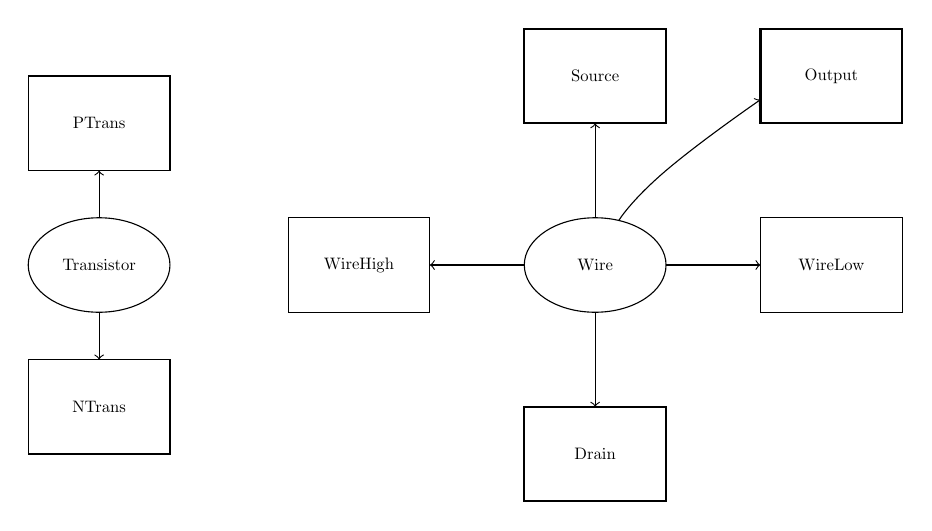
\begin{tikzpicture}[scale=0.6, every node/.style={scale=0.6}]

\draw  (0,0) ellipse (1.5 and 1);
\node at (0,0) {Transistor};
\draw  (-1.5,2) rectangle (1.5,4);
\node at (0,3) {PTrans};
\draw  (-1.5,-2) rectangle (1.5,-4);
\node at (0,-3) {NTrans};
\draw [->] plot[smooth, tension=.7] coordinates {(0,1) (0,2)};
\draw [->] plot[smooth, tension=.7] coordinates {(0,-1) (0,-2)};
\draw  (10.5,0) ellipse (1.5 and 1);
\node at (10.5,0) {Wire};
\draw  (7,-1) rectangle (4,1);
\draw  (14,-1) rectangle (17,1);
\node at (5.5,0) {WireHigh};
\node at (15.5,0) {WireLow};
\draw [thick] (9,5) rectangle (12,3);
\draw [thick] (9,-5) rectangle (12,-3);
\draw [thick] (14,3) rectangle (17,5);
\node at (10.5,4) {Source};
\node at (10.5,-4) {Drain};
\node at (15.5,4) {Output};
\draw  [->] plot[smooth, tension=.9] coordinates {(10.5,1) (10.5,3)};
% x = 10,   y = -(2 sqrt(2))/3
\draw  [->] plot[smooth, tension=.9] coordinates {(9,0) (7,0)};
\draw  [->] plot[smooth, tension=.9] coordinates {(12,0) (14,0)};

\draw  [<-] plot[smooth, tension=.9] coordinates {(10.5,-3) (10.5,-1)};

\draw  [->] plot[smooth, tension=0.9] coordinates {(11, 0.94280904158) (12,2) (14,3.5)};

\end{tikzpicture} 
\end{centering}

\caption{Gate and Wire Class Relations}
\end{figure}


\begin{algorithm}[ht!]
\SetKwInOut{Input}{Input}\SetKwInOut{Output}{Output}\SetKwInOut{SideEffects}{Side
Effects} \SetKwData{prvsGt}{previous-gate}\SetKwData{Result}{Result}\SetKwData{Source}{Source}\SetKwData{Drain}{Drain}

\Input{Expression $E=\bigvee_{i=1}^{n}\left(\bigwedge_{j=1}^{m}P_{i}\right)$
in Disjunctive Normal Form}

\Output{None}

\SideEffects{Transistor network produced on \Result} \BlankLine

clear \Result\; \prvsGt $\gets()$\; \ForEach{$c_{i}\in E=c_{1}\lor c_{2}\lor\ldots\lor c_{n}$}{
\ForEach{$l_{i}\in c_{i}=l_{1}\land l_{2}\land\ldots\land l_{m}$}{
\eIf{\prvsGt is defined}{ Create a new gate and connect it to
\prvsGt, updating \prvsGt to the new gate\; }{ Create a new gate
and connect it to \Result, setting \prvsGt to this gate\; } }
Connect \prvsGt to \Source/\Drain as appropriate\; }

\caption{Converting DNF expression to transistors\label{alg:Converting-DNF-expression}}
\end{algorithm}


The pseudo-code in \vref{alg:Converting-DNF-expression} describes
the final implementation of the gate creation algorithm, however,
initially, a different approach was attempted, which expanded the
number of classes inheriting from \code{Node} to include implications
and a representation of iff, as well as the classes for the transistors.
After parsing the formula, a function then proceeded to try and convert
the formula and its negation into a series of transistors with literals
as inputs, joined by conjunctions and disjunctions. Dealing with the
large number of special cases quickly became impractical, especially
when small repeated changes had to be made, and therefore was abandoned
in favour of a separation of the logical and ``physical'' models,
where the transistors were joined by wires and received potentials
as inputs.

Once an initial array of transistors has been generated, the program
then minimises the number of transistors produced, by traversing from
\code{Source} to \code{Result}, followed by from \code{Drain} to
\code{Result}, looking for transistors operating on the same literal
that may be combined into one group, by removing the redundant transistor,
and extending the wire below, as described in \vref{alg:Minimising-the-transistors}.
Alternatively, rather than working inwards from the outer nodes, it
could work outwards from the \code{Result} wire, however, it is likely
that only one of these passes may be performed, as applying it in
both directions may result in transistors being connected that should
not be, e.g.\ $a\oplus b\oplus c$ will result in $a$ and $\neg a$
being connected to the \code{Souce} twice, and $c$ and $\neg c$
bein connected to the drain twice, however, by merging both sets of
gates, connections are then formed such that \code{Result} is always
driven.

\begin{algorithm}[ht!]
\SetKwInOut{Input}{Input}\SetKwInOut{Output}{Output}\SetKwInOut{SideEffects}{Side
Effects}

\SetKwData{Result}{Result}\SetKwData{totalGates}{total-gates}
\Input{Starting wire, top/bottom network indicator} \Output{None}
\SideEffects{Minimised number of transistors in network\\Updated
totals to reflect this} \BlankLine \If{wire $\neq$ \Result}{
$\mathit{gates}:\mathcal{V}\rightarrow\text{Transistor}\gets\emptyset$\;
\eIf{checkingTopNetwork}{gate-list $\gets$ wire.getDrains}{gate-list
$\gets$ wire.getSources} \ForEach{gate $\in$ gate-list}{ \eIf{$\text{gate.input}\in\mathrm{dom}(\mathit{gates})$}{
\eIf{checkingTopNetwork}{ \ForEach{drain $\in$ gate.drain.getDrains}{gates(gate.input).drain.addDrain(drain)}
}{ \ForEach{source $\in$ gate.source.getSources}{gates(gate.input).source.addSource(source)}
} remove gate\; $\totalGates\gets\totalGates-1$\; }{ $\mathit{gates}\gets\mathit{gates}\cup\{(gate.input,gate)\}$\;
} } }

\caption{Minimising the number of transistors\label{alg:Minimising-the-transistors}}
\end{algorithm}


Additionally, it may be more expedient to negate the expression that
needs finding and then negate the output to determine a final drivenness
result, as if several input variables need negating, this will require
an extra two transistors per variable. For example, $a\land b$ requires
8 gates ($\neg a$ from \code{Source} to intermediate wire, $\neg b$
from intermediate wire to \code{Result}, $\neg a$ from \code{Drain}
to \code{Result}, $\neg b$ from \code{Drain} to \code{Result},
and a pair of transistors to produce each of $\neg a$, and $\neg b$),
whereas $\neg(\neg a\lor\neg b)$ requires 6 transistors ($a$ from
\code{Drain} to intermediate wire, $b$ from intermediate wire to
\code{Result}, $a$ from \code{Source} to \code{Result}, $b$ from
\code{Source} to \code{Result}, and a pair of transistors to produce
the final negation). It is therefore necessary to generate the transistor
networks at least twice, however, it is far more useful to the program's
structure to implement \code{Result} as a single static object, and
in half of the cases, the worst-case of three passes will not be needed.
This is discussed in more detail in \vref{alg:Determining-the-optimal}.

\begin{algorithm}[ht!]
\SetKwInOut{Input}{Input}\SetKwInOut{Output}{Output}\SetKwInOut{SideEffects}{Side
Effects}

\SetKwFunction{tryLayout}{try-layout}\SetKwData{expr}{expr}\SetKwData{Result}{Result}
\Input{Expression to convert to transistors \expr} 
\Output{Integer value of number of gates needed}
\SideEffects{Transistor network produced on \Result}
\BlankLine 

$\text{normal}\gets\tryLayout{\expr}$\;

$\text{double-negate}\gets\tryLayout{$\neg\expr$} + 2$\;

\eIf{$\text{normal}\le\text{doubleNegate}$} { 
	\tryLayout{\expr}\; \Return normal\; 
} { 
	\Return double-negate\; 
}

\caption{Determining the optimal sequence of negations\label{alg:Determining-the-optimal}}
\end{algorithm}


Initially, potential was going to be simulated using the \code{Option{[}Boolean{]}} type,
with \code{Some(true)} and \code{Some(false)} to indicate high and
low potential separately, and \code{Nothing} to simulate a transistor or wire that is not driven.
This approach has also been reworked, to
further separate the differences between the abstract logical expressions
with precise true/false values, and the CMOS-specific high and low
potentials where the transistors/wires are driven, or a specific \code{Undriven}
value. Functionally, this does not differ significantly in practise
from the originally proposed \code{Option{[}Boolean{]}} implementation.
The pseudo-code in \vref{alg:Traversing-transistors-to}, and \vref{alg:Helper-methods-Drivenness}
describe in further detail the steps required to determine drivenness.

\begin{algorithm}[ht!]
\SetKwInOut{Input}{Input}\SetKwInOut{Output}{Output}\SetKwInOut{SideEffects}{Side
Effects} \SetKwData{prvsGt}{previous-transistor}\SetKwData{Result}{Result}\SetKwData{Source}{Source}\SetKwData{Drain}{Drain}
\SetKwData{ptransistor}{P-transistor}\SetKwData{ntransistor}{N-transistor}\SetKwData{wh}{WireHigh}\SetKwData{wl}{WireLow}
\SetKwData{high}{High}\SetKwData{low}{Low}\SetKwData{und}{Undriven}\SetKwFunction{gstatus}{transistor-Status}\SetKwFunction{wstatus}{Wire-Status}
\SetKwProg{Def}{def}{ as}{end} \Input{None (necessary information
contained in static object)} \Output{True/false value to indicate
if the output is driven} \SideEffects{None} \BlankLine $r\gets\und$\;
\ForEach{transistor $\in$ \Result sources}{ \If{$\gstatus{gate}\neq\und$}{$r\gets$
\gstatus{transistor}\;} } \If{$r=\und$}{ \ForEach{transistor
$\in$ \Result drains}{ \If{$\gstatus{gate}\neq\und$}{$r\gets$
\gstatus{transistor}\;} } } \eIf{$r=\und$}{report error}{\Return
$r$}

\caption{Traversing transistors to determine drivenness\label{alg:Traversing-transistors-to}}
\end{algorithm}


\begin{algorithm}[ht!]
\SetKwInOut{Input}{Input}\SetKwInOut{Output}{Output} \SetKwData{prvsGt}{previous-transistor}\SetKwData{Result}{Result}\SetKwData{Source}{Source}\SetKwData{Drain}{Drain}
\SetKwData{ptransistor}{P-transistor}\SetKwData{ntransistor}{N-transistor}\SetKwData{wh}{WireHigh}\SetKwData{wl}{WireLow}
\SetKwData{high}{High}\SetKwData{low}{Low}\SetKwData{und}{Undriven}\SetKwFunction{gstatus}{transistor-Status}\SetKwFunction{wstatus}{Wire-Status}
\SetKwProg{Def}{def}{ as}{end} \Def{\gstatus(transistor:
Transistor)}{ \Input{transistor to check for drivenness} \Output{Potential
on transistor} $r\gets\und$\; \eIf{transistor is \ptransistor}{
\eIf{$\neg$transistor.input}{$r\gets$\wstatus{transistor.source}}{$r\gets\und$}
}{ By symmetry for \ntransistor } \Return $r$\; } \Def{\wstatus(wire:
Wire)}{ \Input{wire to check for driven-ness} \Output{Potential
on wire} $r\gets\und$\; \If{wire is \Source}{$r\gets\high$}
\ElseIf{wire is \Drain}{$r\gets\low$} \ElseIf{wire is \wh}{
\eIf{$\neg$transistor.input}{$r\gets$\wstatus{transistor.source}}{$r\gets\und$}
}\ElseIf{wire is \wl}{ By symmetry for \wl } \Return $r$\;
}

\caption{Helper methods to determine drivenness\label{alg:Helper-methods-Drivenness}}
\end{algorithm}



\subsubsection{Helpers}


\paragraph{Parsing\label{sub:Parsing}}

The Packrat parsing library is one of the many libraries available
in Scala for parsing purposes.\cite{packrat} This library has the
advantage of allowing efficient parsing by using memoization to reduce
the number of times that a production rule needs testing. This parsing
library uses a domain-specific language to assist in the definition
of the grammar to be parsed to ensure that the abstract representation
of the grammar matches the implementation as closely as possible.


\paragraph{Normal Forms\label{sub:Normal-Forms}}

After an expression is parsed, it is then converted to a normal form
to allow the transistor conversion tool to process it, in this case,
as a disjunction of conjunctions, by using the Quine-McCluskey Algorithm,
and algorithm developed by McCluskey\cite{mccluskey}, building on
work by Quine\cite{quine1,quine2}. The algorithm has the following
sections: 
\begin{enumerate}
\item Convert logical expression to boolean function: 
\begin{eqnarray*}
f & : & \{0,1\}^{\mid\mathcal{A}\mid}\rightarrow\{0,1\}\\
f\left(v_{1},v_{2},\ldots v_{n}\right) & = & \sum m\left(n_{1},n_{2},\ldots,n_{m}\right)+d\left(n_{m+1},\ldots,n_{k}\right)
\end{eqnarray*}
where $m$ is the set of minterms, and $d$ is the set of ``don't
care'' values (not needed in this implementation, as we are only
considering logical expressions that are defined in the syntax given
above). The minterms give a non-minimal canonical representation of
a formula (e.g.\ for $f(A,B)=\sum m(0)$, $f$ represents the boolean
formula $\neg A\land\neg B$). This is described in more detail in
\vref{alg:Quine-McCluskey----Logical}. 
\item Find the prime implicants of the function ($P$ is an \emph{implicant}
for $F$ if $P$ is a conjunction of literals, and if $\mathcal{A}\models F$
whenever$\mathcal{A}\models P$. A \emph{prime implicant} is an implicant
that is minimal in the number of terms that it contains (i.e.\ no
more literals can be removed without it becoming a non-implicant)).
This is described in more detail in \vref{alg:Quine-McCluskey----Prime}. 
\item Find the essential prime implicants, as well as any others that are
necessary to cover the function (a prime implicant is \emph{essential
}when it is the only prime implicant to cover some minterm). This
is described in more detail in \vref{alg:Quine-McCluskey----Essential}. 
\item Print/export the results using the list of variables to assign values,
and iterating through each of the essential implicants. This will
also result in the returned expression's clauses already being in
alphabetical order, making later optimisations based on connections
of gates easier. 
\end{enumerate}
\begin{algorithm}[ht!]
\SetKwInOut{Input}{Input}\SetKwInOut{Output}{Output}\SetKwData{expr}{Expression}
\SetKwData{mts}{Minterms} \Input{Logical Expression} \Output{List
of minterms} \BlankLine Get from $\mathcal{V}$ from \expr\; Variable
list $\gets$ ``''\; \ForEach{$v\gets\mathcal{V}$}{Variable
list $\gets v+\text{Variable list}$\;}

\ForEach{$i\in\{0,1,\ldots,2^{\mid\mathcal{V}\mid}\}$}{ \ForEach{$j\in\mathbb{Z}_{\mid\mathcal{V}\mid}$}{$\mathcal{A}\left(v_{j}\right)=\sfrac{i}{2^{j}}\mod2$\;}
\If{$\mathcal{A}\models\expr$}{\mts $\gets\mts\cup\{i\}$}
} \Return \mts

\caption{Quine-McCluskey -- Logical Expression to Boolean Function\label{alg:Quine-McCluskey----Logical}}
\end{algorithm}


\begin{algorithm}[ht!]
\SetKwInOut{Input}{Input}\SetKwInOut{Output}{Output}\SetKwData{expr}{Expression}
\SetKwData{mts}{minterms}\SetKwData{imtbl}{implicant-table}
\Input{List of minterms \mts} \Output{List of prime implicants}
\BlankLine \ForEach{$i\in\mts$}{ $\text{trueCount}=0$\; \ForEach{$j\in\mathbb{Z}_{\mid\mathcal{V}\mid}$}{
$\imtbl_{i,v_{j}}\gets\sfrac{i}{2^{j}}\mod2$\; $\text{trueCount}\gets\text{trueCount}+\sfrac{i}{2^{j}}\mod2$\;
} $\imtbl_{i,\text{trueCount}}\gets\text{trueCount}$\; } $\text{modified}\gets\top$\;
\While{$\text{modified}=\top$}{ $\text{modified}\gets\bot$\;
\ForEach{$i\in\imtbl$}{ \ForEach{$j\in\imtbl,j\neq i$}{
\If{$i$ and $j$ differ in one position in \imtbl}{ $\imtbl_{\langle i,j\rangle}\gets\imtbl_{i}\oplus\imtbl_{j}$
where $i\oplus j$ produces $i\land j$ with any differences replaced
with --\; $\text{modified}\gets\top$\; } } \If{$\text{modified}=\bot$}{
mark $i$ as prime\; } } } \Return marked entries in \imtbl\caption{Quine-McCluskey -- Prime Implicants\label{alg:Quine-McCluskey----Prime}}
\end{algorithm}


\begin{algorithm}[ht!]
\SetKwInOut{Input}{Input}\SetKwInOut{Output}{Output}\SetKwData{expr}{Expression}
\SetKwData{mts}{Minterms}\SetKwData{pimps}{prime-implicants}\SetKwData{mtsimp}{minterm-imp-table}
\SetKwData{mmts}{minimised-minterms}\SetKwData{cmts}{covered-minterms}\SetKwData{cimps}{chosen-implicants}
\Input{List of prime implicants, and minterms} \Output{Minimised
expression in DNF} \BlankLine \ForEach{$m\in\mts$}{ \ForEach{$p\in\pimps$}{
\If{$m\models p$}{ $\mtsimp_{m,p}\gets\top$\; } } } \BlankLine
$\cmts\gets\emptyset$\; $\cimps\gets\emptyset$\; \ForEach{$m\in\mts$}{
\If{$\mid x=\{i\in\mtsimp:\mtsimp_{m,i}=\top\}\mid=1$}{ $\mmts\gets\mmts\cup x$\;
\ForEach(Find all essential implicants, and add them to the list
of required implicants){$\text{minterm}\in x$} { $\cmts\gets\cmts\cup\text{minterm}$\;
} } } \BlankLine \ForEach{$m\in\mts\setminus\cmts$}{ Find
$c\in\pimps$ such that $c$ covers $m$ and as many other values
as possible\; $\mmts\gets\mmts\cup\{c\}$\; } \Return \mmts

\caption{Quine-McCluskey -- Essential and covering implicants\label{alg:Quine-McCluskey----Essential}}
\end{algorithm}


When processing a logical expression by hand, the usual method is
to produce a Karnaugh map, first discussed in \cite{karnaugh}, and
use manual techniques to quickly find minterms that cover as much
as possible. For example, the Karnaugh maps for $(a\land b)\lor(\neg a\land\neg b\land c)$,
and $a\oplus b\oplus c$ are produced in \vref{tab:Karnaugh-Maps}.
While the first expression, and its negation, decomposes nicely into
a series of clauses where each clause covers at least one other box,
and usually two, $a\oplus b\oplus c$ is an example of a degenerate
case without any such nice decomposition, but rather, each clause
produced covers one box at a time.

\begin{table}
\begin{centering}
\begin{tabular}{ccc}
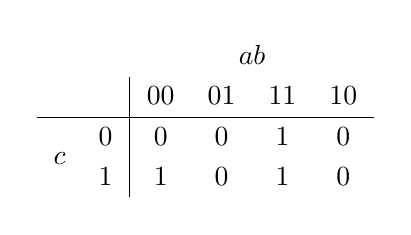
\begin{tikzpicture}
\node (table) {\begin{tabular}{cc|cccc}
 & \multicolumn{1}{c}{} & \multicolumn{4}{c}{$ab$}\tabularnewline
 &  & 00 & 01 & 11 & 10\tabularnewline
\hline
\multirow{2}{*}{$c$} & 0 & 0 & 0 & 1 & 0\tabularnewline
 & 1 & 1 & 0 & 1 & 0\tabularnewline
\end{tabular}
};

\end{tikzpicture} &  & 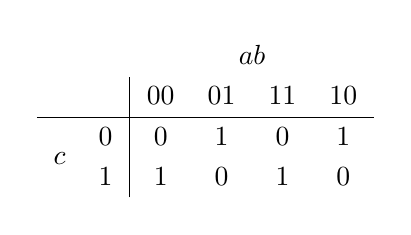
\begin{tikzpicture}
\node (table) {\begin{tabular}{cc|cccc}
 & \multicolumn{1}{c}{} & \multicolumn{4}{c}{$ab$}\tabularnewline
 &  & 00 & 01 & 11 & 10\tabularnewline
\hline
\multirow{2}{*}{$c$} & 0 & 0 & 1 & 0 & 1\tabularnewline
 & 1 & 1 & 0 & 1 & 0\tabularnewline
\end{tabular}
};
\end{tikzpicture}\tabularnewline
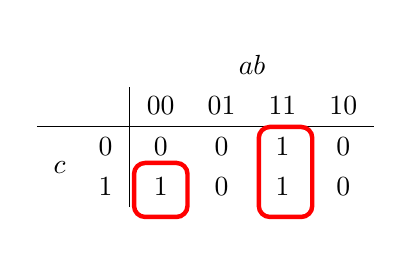
\begin{tikzpicture}
\node (table) {\begin{tabular}{cc|cccc}
 & \multicolumn{1}{c}{} & \multicolumn{4}{c}{$ab$}\tabularnewline
 &  & 00 & 01 & 11 & 10\tabularnewline
\hline
\multirow{2}{*}{$c$} & 0 & 0 & 0 & 1 & 0\tabularnewline
 & 1 & 1 & 0 & 1 & 0\tabularnewline
\end{tabular}
};
\node (topleft)  at ($(table.north west) !.45! (table.north east)$) {};
\node (bottomleft)  at ($(table.south west) !.45! (table.south east)$) {};
\node (topright)  at ($(table.north west) !.8! (table.north east)$) {};
\node (bottomright)  at ($(table.south west) !.8! (table.south east)$) {};
\draw [red, ultra thick,rounded corners]
  ($(table.south west) !.3! (table.south  east)$)
    rectangle
	($(topleft.center) !.7! (bottomleft.center)$);

\draw [red, ultra thick,rounded corners]
  ($(table.south west) !.65! (table.south  east)$)
    rectangle
	($(topright.center) !.5! (bottomright.center)$);


\end{tikzpicture} &  & 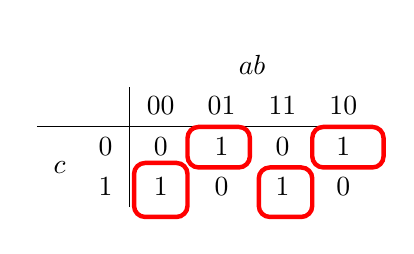
\begin{tikzpicture}
\node (table) {\begin{tabular}{cc|cccc}
 & \multicolumn{1}{c}{} & \multicolumn{4}{c}{$ab$}\tabularnewline
 &  & 00 & 01 & 11 & 10\tabularnewline
\hline
\multirow{2}{*}{$c$} & 0 & 0 & 1 & 0 & 1\tabularnewline
 & 1 & 1 & 0 & 1 & 0\tabularnewline
\end{tabular}
};
\node (topleft)  at ($(table.north west) !.45! (table.north east)$) {};
\node (bottomleft)  at ($(table.south west) !.45! (table.south east)$) {};
\node (topright)  at ($(table.north west) !.8! (table.north east)$) {};
\node (bottomright)  at ($(table.south west) !.8! (table.south east)$) {};
\draw [red, ultra thick,rounded corners]
  ($(table.south west) !.3! (table.south  east)$)
    rectangle
	($(topleft.center) !.7! (bottomleft.center)$);

\draw [red, ultra thick,rounded corners]
	($(topleft.center) !.725! (bottomleft.center)$)
		rectangle
		($(table.east) !.375! (table.west)$);

\draw [red, ultra thick, rounded corners]
    ($(table.south west) !.65! (table.south east)$)
      rectangle
	  ($(topright.center) !.725! (bottomright.center)$);

\draw [red, ultra thick, rounded corners]
	  ($(topright.center) !.725! (bottomright.center)$)
	  rectangle (table.east);
\end{tikzpicture}\tabularnewline
\end{tabular}
\par\end{centering}

\caption{Karnaugh Maps\label{tab:Karnaugh-Maps}}
\end{table}



\subsection{View and Controller}

The view and controller are handled by two separate classes, one with
an overall responsibility for drawing and updating the UI view presented
to the user, written in Java and named \code{Gui}, which then invokes
the \code{DrawCircuit} Scala class to initially draw and then update
the displayed circuit as the inputs are changed. The following algorithm
is a na\"{i}ve version, designed for drawing transistors where each
wire, other than the static \code{Source}, \code{Drain}, and \code{Result}
has precisely one transistor attached. This is described in more detail
in \vref{alg:Transistor-Drawing-Algorithm}.

\begin{algorithm}[ht!]
\SetKwInOut{Input}{Input}\SetKwInOut{Output}{Output}\SetKwInOut{SideEffects}{Side
Effects} \SetKwData{prvsGt}{previous-transistor}\SetKwData{Result}{Result}\SetKwData{Source}{Source}\SetKwData{Drain}{Drain}
\SetKwData{graph}{Graph}\SetKwData{ntransistor}{N-transistor}\SetKwData{ptransistor}{P-transistor}\SetKwData{lasttransistors}{last-transistors}
\SetKwFunction{gstatus}{transistor-Status}\SetKwData{und}{Undriven}
\Input{Graph object to modify}
\Output{None} \SideEffects{Graph updated with visual representation
of transistors} \BlankLine

Clear \graph\;

Add \Result to graph as long thin horizontal line going through $(0,0)$\;

$x\leftarrow0$\;

\ForEach{transistor : \ntransistor attached to \Result}{

$y\leftarrow0$\;

current-transistor $\leftarrow$ transistor\;

\While{current-transistor $\neq$ \Source}{

Add current-transistor to \graph at $(x,y)$ with size $(\delta_{x},\delta_{y})$\;

\If{\gstatus{current-transistor}$\neq\und$}{Highlight current-transistor}

current-transistor $\leftarrow$ transistor.next\;

$y\leftarrow y+\delta_{y}$\;

}

\lasttransistors $\leftarrow$ \lasttransistors $\cup$ current-transistor\;

$x\leftarrow x+\delta_{x}$\;

}

The above, by symmetry, for the bottom transistor network\;

\ForEach{transistor $\in$ \lasttransistors}{

\eIf{transistor : \ntransistor}{

Connect transistor to \Source\;

}{

Connect transistor to \Drain\;

} }

\caption{Transistor Drawing Algorithm\label{alg:Transistor-Drawing-Algorithm}}
\end{algorithm}


In order to modify the above algorithm to draw transistors where one
wire may have multiple transistors attached, the drawing algorithm
checks for the presence of a pre-drawn transistor, and if it is found,
connects the two branches and finishes drawing (as it would otherwise
duplicate work). This does increase the work necessary before drawing,
however, as the presence of drawn transistors needs to be removed,
using a visitation pattern not dissimilar to the method used to determine
drivenness. This is described in more detail in \vref{alg:Optimised-Transistor-Drawing}.

\begin{algorithm}[ht!]
\SetKwInOut{Input}{Input}\SetKwInOut{Output}{Output}\SetKwInOut{SideEffects}{Side
Effects} \SetKwData{prvsGt}{previous-transistor}\SetKwData{Result}{Result}\SetKwData{Source}{Source}\SetKwData{Drain}{Drain}
\SetKwData{graph}{Graph}\SetKwData{ntransistor}{N-transistor}\SetKwData{ptransistor}{P-transistor}\SetKwData{lasttransistors}{last-transistors}\SetKwData{drawntransistors}{drawn-transistors}
\SetKwFunction{gstatus}{transistor-Status}\SetKwData{und}{Undriven}
\Input{Graph object to modify}
\Output{None} \SideEffects{Graph updated with visual representation
of transistors} \BlankLine

Clear \graph\;

Traverse transistors to reset drawn-transistor property\;

$\drawntransistors\gets\emptyset$\;

Add \Result to graph as long thin horizontal line going through $(0,0)$\;

$x\leftarrow0$\;

\ForEach{transistor : \ntransistor attached to \Result}{

$y\leftarrow0$\;

current-transistor $\leftarrow$ transistor\;

\While{current-transistor $\neq$ \Source}{

\eIf{current-transistor.drawn-node$=\emptyset$}{

Add current-transistor to \graph at $(x,y)$ with size $(\delta_{x},\delta_{y})$\;

$\drawntransistors\gets\drawntransistors\cup\{\text{current-transistor}\}$\;

\If{\gstatus{current-transistor}$\neq\und$}{Highlight current-transistor}

current-transistor $\leftarrow$ transistor.next\;

$y\leftarrow y+\delta_{y}$\;

}{ Connect \prvsGt to current-transistor.drawn-node\; current-transistor$\gets\Source$\;
} }

\lasttransistors $\leftarrow$ \lasttransistors $\cup$ current-transistor\;

$x\leftarrow x+\delta_{x}$\;

}

The above, by symmetry, for the bottom transistor network\;

\ForEach{transistor $\in$ \lasttransistors}{

\eIf{transistor : \ntransistor}{

Connect transistor to \Source\;

}{

Connect transistor to \Drain\;

} }

\caption{Optimised Transistor Drawing Algorithm\label{alg:Optimised-Transistor-Drawing}}
\end{algorithm}


Unfortunately, this algorithm does not properly take into account
overlapping transistors/wires, as they are drawn from the \code{Result}
wire outwards. Techniques to allow both the optimised drawing algorithm,
and the gate-reduction algorithms to work together more effectively
are discussed in \vref{sec:Conclusions-and-Further}.


\section{Comparison to a Compiler}

The usual definition of a compiler is ``a program that can read a
program in one language and translate it into an equivalent program
in another language'' \cite{aho2003compilers} usually with some
sort of intermediate feedback if errors are encountered; with most
compilers usually translating from a human-readable, high-level language
into something low-level that can then be directly executed by a machine.
The structure of a compiler can be thought of as the composition of
a series of functions, each with a distinct focus, as shown in \prettyref{fig:Compiler-Structure}.

\begin{figure}
\begin{centering}
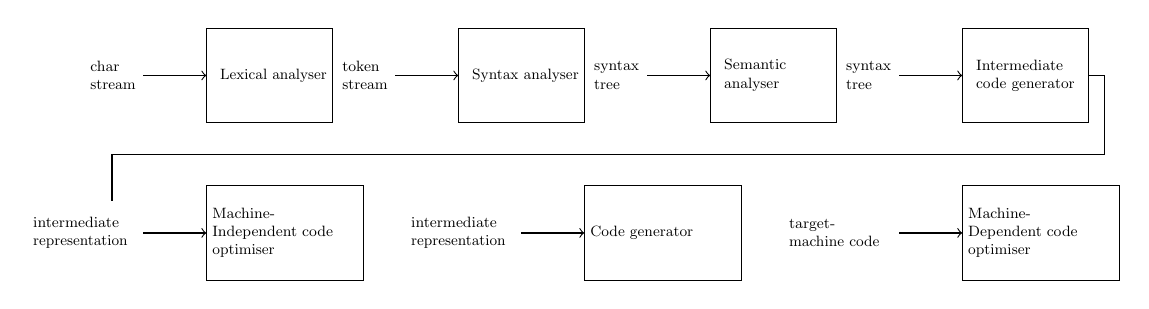
\begin{tikzpicture}[scale=0.4, every node/.style={x=1cm,y=1cm,scale=0.6,font=\small}]

\def\type{{"char stream","token stream","syntax tree","syntax tree","intermediate representation","intermediate representation","target-machine code","target-machine code"}}%

\def\function{{"Lexical analyser","Syntax analyser","Semantic analyser","Intermediate code generator","Machine-Independent code optimiser","Code generator","Machine-Dependent code optimiser"}}%

\foreach \i in {0,8,16,24} {
	\draw (\i,0) rectangle (\i+4,3);
	\draw [->] plot coordinates{ (\i-2,1.5)  (\i,1.5) };
	\node [text width=2.25cm] at (\i+2.125, 1.5) {\pgfmathparse{\function[\i/8]}\pgfmathresult};
	\node [text width=1.25cm] at (\i-2.75, 1.5) {\pgfmathparse{\type[\i/8]}\pgfmathresult};
}

\foreach \i in {0,12,24} {
	\draw (\i,-5) rectangle (\i+5,-2);
	\draw [->] plot coordinates{ (\i-2,-3.5)  (\i,-3.5) };
	\node [text width=2.75cm] at (\i+2.25, -3.5) {\pgfmathparse{\function[\i/12+4]}\pgfmathresult};
	\node [text width=2cm] at (\i-4, -3.5) {\pgfmathparse{\type[\i/12+4]}\pgfmathresult};
}
\draw (28,1.5) -- (28.5,1.5) -- (28.5,-1) -- (-3,-1) -> (-3,-2.5);
\end{tikzpicture}
\par\end{centering}

\caption{Compiler Structure\label{fig:Compiler-Structure}}
\end{figure}


In a conventional compiler, the lexical analysis stage splits up the
entered text into variables to be recognised within the program, or
as keywords/reserved tokens within the language, usually achieved
using some deterministic finite automata to recognise a regular expression,
with some order of precedence established to allow keywords to be
treated as such, rather than as variables. This is followed by syntax
analysis, where the discrete tokens are then used to form a \emph{syntax
tree}, where the nodes are production rules or terminals in the context-free
grammar, and the edges correspond to variables leading to further
production rules, similar to the structure of logical expressions
defined in \eqref{eq:neg} to \eqref{eq:var} in \vref{eq:cons}.
Semantic analysis varies in its depth, depending on the language,
however, most compilers will usually perform some sort of check for
proper declaration, as well as ensuring that variables are not used
outside of the scope that they were defined in.

The lexical, syntax, and semantic analysis stages can all be thought
to be covered by the parsing stages in the application, as the various
tokens in the language (\code{and}, \code{or}, \code{!}, \code{(},
and \code{)}) are isolated and then used to form the syntax tree,
while variables are added to the assignment map in the \code{Variable}
object. Additionally, should any stage of the parsing module fail,
the first of these errors is then reported back to the user to allow
them to correct their input, and the assignment map emptied so that
their previous state does not then affect their next input. Owing
to the simplicity of the propositional logic language, there is obviously
no need for formal semantic analysis of the entered expression, however,
it is useful to register each variable, with the minimal semantic
check that the reserved keywords \code{out}, \texttt{and}, and \texttt{or}
are not used in the entered expression.

Once no more work can occur on the syntax tree, the compiler then
starts to focus on generating code, directed by the structure of the
syntax tree, following by platform-agnostic optimisations that focus
on repeated patterns within the code, or redundant operations often
focusing on a small number of operations at any one time. This process
is often called \emph{peep-hole optimisation} owing to the metaphor
of only being able to see a small part of a scene at any one time
through a peep-hole camera.

This is replaced in the CMOS calculator by the Quine-McCluskey algorithm
before transistor generation, effectively putting the optimisation
before the code generation, though in a more general software engineering
metaphor, this could be considered as a refactoring to remove redundancy
before actually compiling the code, resulting in different byte-code,
but with equivalent effects. Additionally, this has the advantage
of ensuring that expressions such as $\bigwedge_{i=0}^{n}a$ get reduced
properly to $a$, rather than attempting to produce $n$ N-transistors
in series for , followed by $n$ P-transistors in parallel, so the
number of gates is strictly bound by the number of variables, rather
than the size of the entered expression.

Once no more work can take place on the intermediate code, a compiler
then starts producing platform-specific code, followed by any further
platform-specific operations. In the CMOS calculator's case, this
would then be the transistor generation algorithm, taking the canonical
form generated by the Quine-McCluskey algorithm, and turning it into
the CMOS implementation.

The next stage in the pipeline produces optimisations to the machine-readable
code that has been produced for the relevant platform, with a specific
focus on architecture specific optimisations. For Intel-based systems,
with their larger instruction sets, and instructions capable of processing
multiple operations on data at a time, this may focus on maximising
the number of pieces of data operated upon by combining them into
vectors, or on ARM machines with large numbers of registers, this
frequently translates into taking advantage of the large caches available
to minimise the number of secondary memory lookups and therefore the
number of cycles spent idling while the RAM is queried. Within the
context of the CMOS transistors, this then focuses on maximising the
number of transistors that may be eliminated while retaining the same
original expression. Just as the optimisation stages of a compiler
will focus on the structure of the program to find subtle optimisations,
so too does this program produce a minimised final output by examining
the wires nearest to it.


\section{Testing}


\subsection{General Testing Strategy}

The output from the logical expression classes was deliberately designed
so that the output that they would produce would be compatible with
the parser, thus making testing the output of any given module producing
logical expressions as output much easier, as they could then be compared
to the expected values, once the behaviour of the parser was verified.

Where possible the testing is designed to test error cases, simple
cases (e.g. atoms in the parser, or simple expressions for the Quine-McCluskey
algorithm), followed by more complicated cases, usually based on the
inductive definitions seen above.


\subsection{Parsing}

Care must be taken, as already discussed to ensure that only valid
inputs are parsed, without affecting the ability of the program to
operate using predefined constants that have been set aside for specific
purposes. Furthermore, the parser must ensure that statements are
parsed with due care paid to the order of operations, with negations
binding correctly. The contents of \vref{tab:Parsing-Test-Data} list
the sample test data and expected outcomes.

\begin{table}
\begin{centering}\small
\begin{tabularx}{\linewidth}{@{}lX@{}}
            \toprule
Input       & Expected Output                         \tabularnewline
            \midrule
``''        & None                                    \tabularnewline
0           & False                                   \tabularnewline
1           & True                                    \tabularnewline
out         & None                                    \tabularnewline
test        & Variable(test)                          \tabularnewline
(           & None                                    \tabularnewline
)           & None                                    \tabularnewline
()          & None                                    \tabularnewline
a           & Variable(a)                             \tabularnewline
(a)         & Variable(a)                             \tabularnewline
!           & None                                    \tabularnewline
!a          & Not(Variable(a))                        \tabularnewline
(!a)        & Not(Variable(a))                        \tabularnewline
!(a)        & Not(Variable(a))                        \tabularnewline
and         & None                                    \tabularnewline
a and       & None                                    \tabularnewline
and a       & None                                    \tabularnewline
a and b     & And(Variable(a), Variable(b))           \tabularnewline
!a and b    & Not(And(Variable(a), Variable(b))       \tabularnewline
a and !b    & And(Variable(a), Not(Variable(b)))      \tabularnewline
!a and !b   & Not(And(Variable(a), Not(Variable(b)))  \tabularnewline
(!a) and b  & And(Not(Variable(a)), Variable(b))      \tabularnewline
a and (!b)  & And(Variable(a), Not(Variable(b)))      \tabularnewline
(!a) and !b & And(Not(Variable(a)), Not(Variable(b))) \tabularnewline
or          & None                                    \tabularnewline
a or        & None                                    \tabularnewline
or a        & None                                    \tabularnewline
a or b      & Or(Variable(a), Variable(b))            \tabularnewline
!a or b     & Not(Or(Variable(a), Variable(b)))       \tabularnewline
a or !b     & Or(Variable(a), Not(Variable(b)))       \tabularnewline
!a or !b    & Not(Or(Variable(a), Not(Variable(b))))  \tabularnewline
(!a) or b   & Or(Not(Variable(a)), Variable(b))       \tabularnewline
a or (!b)   & Or(Variable(a), Not(Variable(b)))       \tabularnewline
(!a) or !b  & Or(Not(Variable(a)), Not(Variable(b)))) \tabularnewline \bottomrule
\end{tabularx}
\par\end{centering}
\normalsize

\caption{Parsing Test Data\label{tab:Parsing-Test-Data}}
\end{table}



\subsection{Quine-McCluskey Algorithm}

The contents of \vref{tab:QMA-Test-Data} list the sample test data
and expected outcomes.

\begin{table}
\begin{centering}\small
\begin{tabularx}{\linewidth}{@{}lX@{}}
                                      \toprule
Input                                 & Expected Output                                                                                                         \tabularnewline
                                      \midrule
(!a) and a                            & None                                                                                                                    \tabularnewline
(!a) or a                             & None                                                                                                                    \tabularnewline
a and and a and a                     & Variable(a)                                                                                                             \tabularnewline
a or a or a or a                      & Variable(a)                                                                                                             \tabularnewline
((!a) and b) or (a and (!b))          & Or(And(Variable(a),  Not(Variable(b))),  And(Not(Variable(a)),  Variable(b)))                                           \tabularnewline
!((a and b) or ((!a) and (!b) and c)) & Or(Or(And(Not(Variable(b)), Variable(a)), And(Not(Variable(c)), Not(Variable(a)))), And(Variable(b), Not(Variable(a)))) \tabularnewline
a and b and c                         & And(Variable(c), And(Variable(b), Variable(a)))                                                                         \tabularnewline
c and b and a                         & And(Variable(c), And(Variable(b), Variable(a)))                                                                         \tabularnewline
(a and b and c) or (a and b and c)    & And(Variable(c), And(Variable(b), Variable(a)))                                                                         \tabularnewline
                                      \bottomrule
\end{tabularx}
\par\end{centering}
\normalsize

\caption{Quine-McCluskey Algorithm Test Data\label{tab:QMA-Test-Data}}
\end{table}



\subsection{Transistor Generation and Drawing}

Due to the subjective nature of a ``good'' layout, the diagrams in \vref{tab:vis}
demonstrate the result of entering the following expressions.  When the number of
transistors needed is formatted as $n+2$, this is used to indicate that less transistors
are needed to produce the negation of the expression and negate this, rather than
to produce the original expression.  For clarity, in the case of a tie, the original
expression is preferred.  The visual output shown is used to demonstrate the difference
between the networks of transistors when the output is driven high or driven low, with
arbitrary assignments used to indicate this.
\begin{center}
\begin{table}
\begin{tabularx}{\linewidth}{XXXc}
\toprule 
Input                                      & Driven Output                                  & Undriven Output                                 & Transistors \\
\midrule
$\neg a$                                   & 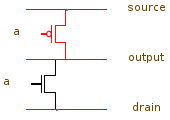
\includegraphics[width=\linewidth]{notdriven}  & 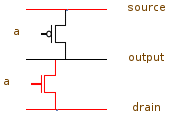
\includegraphics[width=\linewidth]{notundriven} & 2 \tabularnewline
$(a\land b)\lor(\neg a\land\neg b\land c)$ & 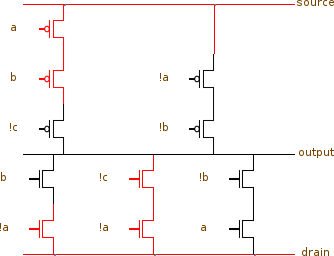
\includegraphics[width=\linewidth]{networklow} & 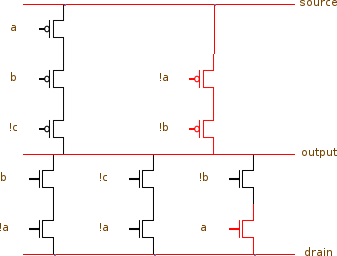
\includegraphics[width=\linewidth]{networkhigh} & 17 \tabularnewline
$a \land b \land c$                        & 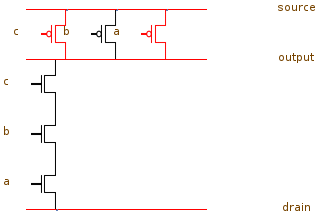
\includegraphics[width=\linewidth]{conjhigh}   & 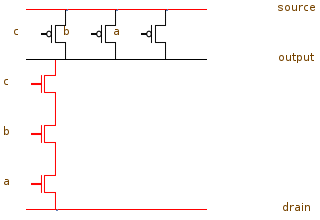
\includegraphics[width=\linewidth]{conjlow}     & $6+2$ \tabularnewline
$a \lor b \lor c$                        & 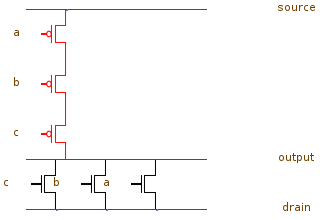
\includegraphics[width=\linewidth]{disjhigh}   & 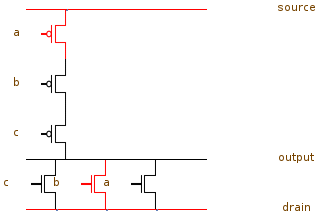
\includegraphics[width=\linewidth]{disjlow}     & $6+2$ \tabularnewline
                                           &                                                & \tabularnewline
                                           &                                                & \tabularnewline
                                           &                                                & \tabularnewline
\bottomrule
\end{tabularx}
\caption{Program Output\label{tab:vis}}
\end{table}
\end{center}
\section{Conclusions and Further Work\label{sec:Conclusions-and-Further}}
\subsection{Conclusions}

The project has achieved much of the scope that it had originally
set out to, however, the order of completion of different subcomponents
of the program needed changing quite substantially. Initially, the
order of completion of the modules was intended to be parser, transistor-generator,
gate-drawer, optimisations (including Quine-McCluskey-related functions),
however, it quickly became apparent that laying out the transistors
would be far quicker and simpler if the input was in some sort of
normal form first, therefore, finding an implementation of the Quine-McCluskey
algorithm became a far higher priority, with drawing and a finalised
transistor-generation algorithm being slightly delayed. On the other
hand, as predicted, once a gate-drawing algorithm was in place, it
became far easier to troubleshoot issues relating to local optimisation
of gates, as the output of the optimisation sequence was far easier
to visualise, rather than attempting to traverse the representation
of wires and transistors stored in the currently executing program's
memory. 
\begin{description}
\item [{Accuracy}] The program's visual output, as the drawing algorithm
is structurally based on the representation within the model, the
rendering is accurate. Owing to constraints on the drawing algorithm,
it was necessary to sacrifice an optimal number of gates in lieu of
ensuring that the drawn output remains consistent and easily interpreted:
due to the way that mxGraph positions vertices and edges, any attempts
to reduce overlap would have caused the edges to shift and become
disconnected. 
\item [{Representation}] The program produces a clearly labelled network
of transistors, with driven transistors indicated in red, and undriven
transistors in black. Unlike the diagrams seen in \vref{fig:Standard-nor--and},
wires linking common variables are not shown, to further enhance clarity,
as in more complicated networks, a large number of overlapping wires
may be needed. Additionally, when a variable needs negating, the small
not-gate is not shown, nor are the transistors necessary, as this
would only complicate the number of diagrams needed, as well as their
layout. 
\item [{Portability}] Beyond the bitmap based images that are produced
by the program, which are then easily converted between similar formats,
there is no other output produced by the program, to either allow
reloading old networks, nor raster-based images to allow simple scaling
without loss of resolution. While a number of workarounds exist to
solve the latter problem, through software that is already in existence,
these are likely to produce images that are less than optimally encoded,
as they will not necessarily take into account. Additionally, unlike
9-patch image files, stretching in one dimension will produce a skewed
image, rather than sub-components resizing themselves intelligently. 
\item [{Interactivity}] The program produces several different types of
warning, corresponding to each stage of the compilation, and then
the current runtime state of the circuit. The earliest warning may
be invoked during parsing if a incorrectly parsed expression is seen,
followed by after the completion of the first stage of the Quine-McCluskey
algorithm, if the entered logical expression has a trivial normal
form ($\top\text{ or \ensuremath{\bot}}$). Finally, in the event
that the circuit produced does not always drive the output with a
high or low potential, this will cause a warning to be thrown as it
occurs, however, this may be a transient error, as the circuit should
only be driven high or low at any time. If in the future, it becomes
possible to import pre-produced circuits, some of these may not be
properly formed, so it is a helpful check to have in place, as well
as when prototyping the transistor production algorithm to ensure
that the output was driven consistently. 
\end{description}

\subsection{Further Work}


\subsubsection{Model}

This project has deliberately focused on defining logical expressions
using strictly binary values, and precisely adhering to the standard
rules for laying out CMOS diagrams, without any deviations. It has
been assumed that the output wire will always be driven, with an undriven
state being invalid, whereas the standard tri-state buffer \cite{digsys}gate,
where $\mathit{enb}\rightarrow(\mathit{in}\leftrightarrow\mathit{out})$,
and $\neg\mathit{enb}$ results in the output wire being undriven.

\begin{figure}
\setlength{\unitlength}{0.015\textwidth} 

\begin{centering}
\begin{picture}(25,27)(-2,-3) \begin{thicklines} \multiput(0,0)(0,24){2}{\line(1,0){18}}
\end{thicklines} \multiput(15,21)(0,-6){2}{\ptrans} \multiput(15,3)(0,6){2}{\ntrans}
\put(15,0){\blob} \put(15,24){\blob} \put(-3,9){\makebox(0,0){${\it enb}$}}
\put(3,9){\blob} \put(0,9){\line(1,0){12}} \put(3,9){\line(0,1){6}}
\put(3,15){\line(1,0){4}} \put(11,15){\notgate} \put(5,21){\notgate}
\put(5,21){\line(1,0){7}} \put(-3,21){\makebox(0,0){${\it in}$}}
\put(6,21){\blob} \put(6,21){\line(0,-1){5.7}} \put(6,14.7){\line(0,-1){5.4}}
\put(6,8.7){\line(0,-1){5.7}} \put(6,3){\line(1,0){6}}
\put(12,12){\line(1,0){6}} \put(21,12){\makebox(0,0){${\it out}$}}
\put(15,12){\blob} \end{picture} 
\par\end{centering}

\caption{Tri-state buffer}
\end{figure}


Additionally, the structure of the transistors produced by the transistor
placing algorithm \nameref{alg:Converting-DNF-expression} is more
constrained than the transistors that may be drawn.

Decreasing the verbosity of the required input should also be a priority
for future development. While operators such as $\rightarrow$, $\leftrightarrow$,
$\oplus$ do not add any additional expressiveness to the language,
they are not currently parsed by the parsing module.

Furthermore, exploring limits on the size of the circuits produced
to more accurately simulate the effects of resistance could be a further
expansion for the system, which would also necessitate changes to
the procedure by which the visual output is created in order to facilitate
animation to properly demonstrate the effect of resistance in the
time taken for the current to flow across a transistor or through
wires, assuming non-negligible resistance. A na\"{i}ve approach would
involve the height of series of transistors being artificially limited,
however, this would not take into account the length of connecting
wires.

The model could also be expanded to include a more formalised notion
of Tony Hoare's drivenness analysis\cite{H88:Calculus}, as discussed
in a draft paper, where formulae~\prettyref{eq:pgate} and \prettyref{eq:ngate}
in \vref{eq:pgate} are updated as follows:

\begin{eqnarray}
\delta P(g,s,d) & = & \neg g\land s\land d\land\delta g\rightarrow(\delta s\leftrightarrow\delta d)\label{eq:pgate-1}\\
\delta N(g,s,d) & = & g\land\neg s\land\neg d\land\delta g\rightarrow(\delta s\leftrightarrow\delta d)\label{eq:ngate-1}
\end{eqnarray}
where the presence of $\delta v$ is used to indicate that $v$ is
driven, either high or low, if $\delta v$ also holds.


\subsubsection{View}

The data produced by the view is currently only in a limited number
of bitmap image formats, whereas a future version of this software
should be able to produce a wider variety of formats, and ideally,
especially for reports like this, \LaTeX{}-compatible output, or Dia
compatible output.

A future implementation of the transistor-drawing algorithm should
be reworked in order to draw the transistors from the \code{Source}
and \texttt{Drain} objects respectively, so as to ensure that grouped
transistors are handled properly, without overlapping, however, this
would also require a more detailed knowledge as to the structure and
bounds of the generated network of transistors.


\subsubsection{Controller}

Due to the implementation of the pointer-based mxGraph that I was
using to produce the visual output, it was not possible for the user
to interact with the graph itself directly, rather, and changes to
the assignments or expression triggered a redraw where any changes
were then made visible. In larger graphs, if they were particularly
complicated, this may not have always been particularly obvious, therefore,
a future iteration of this project, a brief highlighting effect should
be considered, in order to further improve visibility. Additionally,
due to the indirect way of accessing nodes in the graph, a useful
addition would be to include the ability to directly interact with
the graph to see the result of changing specific variables.

Adding the ability to drag-and-drop transistors onto the graph, connect
them and derive an expression for a valid arrangement of transistors
would be a logical extension of the current functionality, though
it is likely that any output produced would, unless the number of
variables was limited, not be in any normal form, due to the cost
of running the Quine-McCluskey algorithm (in the worst case, $\left(\mathcal{O}\left(\sfrac{3^{n}}{n}\right)\right)$
prime implicants will be generated alone). Additionally, unless the
graph was encoded with the rules required for valid CMOS structures,
it would be trivial for users to produce graphs that may have undriven
output, which then cannot be validly encoded as a logical expression.


\section{Acknowledgements}

There are a number of people, without whose assistance over the past
year, this project would not have been possible.

Professor Peter Jeavons, my college tutor, both for his support over
the course of my degree and in the past year.

Professor Geraint Jones, my supervisor, for his advice and support,
as well as some of the standard diagrams of the N-transistors and P-transistors seen
in this document.

James Wallis, and Andrew Wright, the other two Computer Science students
in St Anne's, for their unwavering friendship over the last three year, and
continued support.

Matthew Sj\"odin, Eleanor Kirk, Lucy Wright, and Stephen Heap for general support
throughout the project.

The rest of my family and friends, and all others without whom this project would not have been possible.

\bibliographystyle{plain}
\bibliography{citations}

\clearpage
\begin{landscape}
\appendix
\section{Appendix}
\begin{multicols}{2}
\lstlistoflistings
\subsection{Model}
\lstinputlisting[language=scala,caption=And.scala]{../src/model/And.scala}
\lstinputlisting[language=scala,caption=Atom.scala]{../src/model/Atom.scala}
\lstinputlisting[language=scala,caption=Constant.scala]{../src/model/Constant.scala}
\lstinputlisting[language=scala,caption=Drain.scala]{../src/model/Drain.scala}
\lstinputlisting[language=scala,caption=Driven.scala]{../src/model/Driven.scala}
\lstinputlisting[language=scala,caption=High.scala]{../src/model/High.scala}
\lstinputlisting[language=scala,caption=Low.scala]{../src/model/Low.scala}
\lstinputlisting[language=scala,caption=Node.scala]{../src/model/Node.scala}
\lstinputlisting[language=scala,caption=Not.scala]{../src/model/Not.scala}
\lstinputlisting[language=scala,caption=NTrans.scala]{../src/model/NTrans.scala}
\lstinputlisting[language=scala,caption=Or.scala]{../src/model/Or.scala}
\lstinputlisting[language=scala,caption=Potential.scala]{../src/model/Potential.scala}
\lstinputlisting[language=scala,caption=PTrans.scala]{../src/model/PTrans.scala}
\lstinputlisting[language=scala,caption=Result.scala]{../src/model/Result.scala}
\lstinputlisting[language=scala,caption=Source.scala]{../src/model/Source.scala}
\lstinputlisting[language=scala,caption=Transistor.scala]{../src/model/Transistor.scala}
\lstinputlisting[language=scala,caption=Undriven.scala]{../src/model/Undriven.scala}
\lstinputlisting[language=scala,caption=Variable.scala]{../src/model/Variable.scala}
\lstinputlisting[language=scala,caption=WireHigh.scala]{../src/model/WireHigh.scala}
\lstinputlisting[language=scala,caption=WireLow.scala]{../src/model/WireLow.scala}
\lstinputlisting[language=scala,caption=Wire.scala]{../src/model/Wire.scala}
\end{multicols}
\clearpage
\lstinputlisting[language=scala,caption=Implicant.scala]{../src/model/Implicant.scala}
\lstinputlisting[language=scala,caption=LogicalFunction.scala]{../src/model/LogicalFunction.scala}
\lstinputlisting[language=scala,caption=ParserTest.scala]{../src/model/test/ParserTest.scala}
\lstinputlisting[language=scala,caption=PITable.scala]{../src/model/PITable.scala}
\lstinputlisting[language=scala,caption=PrimeImplicant.scala]{../src/model/PrimeImplicant.scala}
\lstinputlisting[language=scala,caption=qmm.scala]{../src/model/qmm.scala}
\lstinputlisting[language=scala,caption=QuineMcCluskeyTest.scala]{../src/model/test/QuineMcCluskeyTest.scala}
\subsection{View}
\lstinputlisting[language=scala,caption=DrawCircuit.scala]{../src/view/DrawCircuit.scala}
\subsection{Controller}
\lstinputlisting[language=java,caption=Gui.java]{../src/controller/Gui.java}
\subsection{Helper}
\lstinputlisting[language=scala,caption=CMOSLayout.scala]{../src/helper/CMOSLayout.scala}
\lstinputlisting[language=scala,mathescape=false,caption=LogicalExpression.scala]{../src/helper/LogicalExpression.scala}
\lstinputlisting[language=scala,caption=Parser.scala]{../src/helper/Parser.scala}
\end{landscape}
\end{document}

